% Options for packages loaded elsewhere
\PassOptionsToPackage{unicode}{hyperref}
\PassOptionsToPackage{hyphens}{url}
%
\documentclass[
  man,floatsintext]{apa6}
\usepackage{amsmath,amssymb}
\usepackage{lmodern}
\usepackage{iftex}
\ifPDFTeX
  \usepackage[T1]{fontenc}
  \usepackage[utf8]{inputenc}
  \usepackage{textcomp} % provide euro and other symbols
\else % if luatex or xetex
  \usepackage{unicode-math}
  \defaultfontfeatures{Scale=MatchLowercase}
  \defaultfontfeatures[\rmfamily]{Ligatures=TeX,Scale=1}
\fi
% Use upquote if available, for straight quotes in verbatim environments
\IfFileExists{upquote.sty}{\usepackage{upquote}}{}
\IfFileExists{microtype.sty}{% use microtype if available
  \usepackage[]{microtype}
  \UseMicrotypeSet[protrusion]{basicmath} % disable protrusion for tt fonts
}{}
\makeatletter
\@ifundefined{KOMAClassName}{% if non-KOMA class
  \IfFileExists{parskip.sty}{%
    \usepackage{parskip}
  }{% else
    \setlength{\parindent}{0pt}
    \setlength{\parskip}{6pt plus 2pt minus 1pt}}
}{% if KOMA class
  \KOMAoptions{parskip=half}}
\makeatother
\usepackage{xcolor}
\IfFileExists{xurl.sty}{\usepackage{xurl}}{} % add URL line breaks if available
\IfFileExists{bookmark.sty}{\usepackage{bookmark}}{\usepackage{hyperref}}
\hypersetup{
  pdftitle={GenSamp: RESULTS},
  pdfauthor={Gleb Furman1, James E. Pustejovsky2, \& Elizabeth Tipton3},
  pdflang={en-EN},
  hidelinks,
  pdfcreator={LaTeX via pandoc}}
\urlstyle{same} % disable monospaced font for URLs
\usepackage{graphicx}
\makeatletter
\def\maxwidth{\ifdim\Gin@nat@width>\linewidth\linewidth\else\Gin@nat@width\fi}
\def\maxheight{\ifdim\Gin@nat@height>\textheight\textheight\else\Gin@nat@height\fi}
\makeatother
% Scale images if necessary, so that they will not overflow the page
% margins by default, and it is still possible to overwrite the defaults
% using explicit options in \includegraphics[width, height, ...]{}
\setkeys{Gin}{width=\maxwidth,height=\maxheight,keepaspectratio}
% Set default figure placement to htbp
\makeatletter
\def\fps@figure{htbp}
\makeatother
\setlength{\emergencystretch}{3em} % prevent overfull lines
\providecommand{\tightlist}{%
  \setlength{\itemsep}{0pt}\setlength{\parskip}{0pt}}
\setcounter{secnumdepth}{-\maxdimen} % remove section numbering
% Make \paragraph and \subparagraph free-standing
\ifx\paragraph\undefined\else
  \let\oldparagraph\paragraph
  \renewcommand{\paragraph}[1]{\oldparagraph{#1}\mbox{}}
\fi
\ifx\subparagraph\undefined\else
  \let\oldsubparagraph\subparagraph
  \renewcommand{\subparagraph}[1]{\oldsubparagraph{#1}\mbox{}}
\fi
\ifLuaTeX
\usepackage[bidi=basic]{babel}
\else
\usepackage[bidi=default]{babel}
\fi
\babelprovide[main,import]{english}
% get rid of language-specific shorthands (see #6817):
\let\LanguageShortHands\languageshorthands
\def\languageshorthands#1{}
% Manuscript styling
\usepackage{upgreek}
\captionsetup{font=singlespacing,justification=justified}

% Table formatting
\usepackage{longtable}
\usepackage{lscape}
% \usepackage[counterclockwise]{rotating}   % Landscape page setup for large tables
\usepackage{multirow}		% Table styling
\usepackage{tabularx}		% Control Column width
\usepackage[flushleft]{threeparttable}	% Allows for three part tables with a specified notes section
\usepackage{threeparttablex}            % Lets threeparttable work with longtable

% Create new environments so endfloat can handle them
% \newenvironment{ltable}
%   {\begin{landscape}\centering\begin{threeparttable}}
%   {\end{threeparttable}\end{landscape}}
\newenvironment{lltable}{\begin{landscape}\centering\begin{ThreePartTable}}{\end{ThreePartTable}\end{landscape}}

% Enables adjusting longtable caption width to table width
% Solution found at http://golatex.de/longtable-mit-caption-so-breit-wie-die-tabelle-t15767.html
\makeatletter
\newcommand\LastLTentrywidth{1em}
\newlength\longtablewidth
\setlength{\longtablewidth}{1in}
\newcommand{\getlongtablewidth}{\begingroup \ifcsname LT@\roman{LT@tables}\endcsname \global\longtablewidth=0pt \renewcommand{\LT@entry}[2]{\global\advance\longtablewidth by ##2\relax\gdef\LastLTentrywidth{##2}}\@nameuse{LT@\roman{LT@tables}} \fi \endgroup}

% \setlength{\parindent}{0.5in}
% \setlength{\parskip}{0pt plus 0pt minus 0pt}

% Overwrite redefinition of paragraph and subparagraph by the default LaTeX template
% See https://github.com/crsh/papaja/issues/292
\makeatletter
\renewcommand{\paragraph}{\@startsection{paragraph}{4}{\parindent}%
  {0\baselineskip \@plus 0.2ex \@minus 0.2ex}%
  {-1em}%
  {\normalfont\normalsize\bfseries\itshape\typesectitle}}

\renewcommand{\subparagraph}[1]{\@startsection{subparagraph}{5}{1em}%
  {0\baselineskip \@plus 0.2ex \@minus 0.2ex}%
  {-\z@\relax}%
  {\normalfont\normalsize\itshape\hspace{\parindent}{#1}\textit{\addperi}}{\relax}}
\makeatother

% \usepackage{etoolbox}
\makeatletter
\patchcmd{\HyOrg@maketitle}
  {\section{\normalfont\normalsize\abstractname}}
  {\section*{\normalfont\normalsize\abstractname}}
  {}{\typeout{Failed to patch abstract.}}
\patchcmd{\HyOrg@maketitle}
  {\section{\protect\normalfont{\@title}}}
  {\section*{\protect\normalfont{\@title}}}
  {}{\typeout{Failed to patch title.}}
\makeatother

\usepackage{xpatch}
\makeatletter
\xapptocmd\appendix
  {\xapptocmd\section
    {\addcontentsline{toc}{section}{\appendixname\ifoneappendix\else~\theappendix\fi\\: #1}}
    {}{\InnerPatchFailed}%
  }
{}{\PatchFailed}
\usepackage{csquotes}
\ifLuaTeX
  \usepackage{selnolig}  % disable illegal ligatures
\fi

\title{GenSamp: RESULTS}
\author{Gleb Furman\textsuperscript{1}, James E. Pustejovsky\textsuperscript{2}, \& Elizabeth Tipton\textsuperscript{3}}
\date{}


\shorttitle{RESULTS}

\authornote{

Correspondence concerning this article should be addressed to Gleb Furman, University of Texas at Austin, SZB 504, 1912 Speedway, Austin, Texas 78712. E-mail: \href{mailto:gleb.furman@utexas.edu}{\nolinkurl{gleb.furman@utexas.edu}}

}

\affiliation{\vspace{0.5cm}\textsuperscript{1} University of Texas at Austin\\\textsuperscript{2} University of Wisconsin-Madison\\\textsuperscript{3} Northwestern University}

\begin{document}
\maketitle

\hypertarget{setup}{%
\section{Setup}\label{setup}}

\hypertarget{packages-and-data}{%
\subsection{Packages and Data}\label{packages-and-data}}

\hypertarget{organize-objects}{%
\subsection{Organize Objects}\label{organize-objects}}

\hypertarget{data-summary}{%
\section{Data Summary}\label{data-summary}}

\hypertarget{covariate-statistics}{%
\subsection{Covariate Statistics}\label{covariate-statistics}}

\hypertarget{continuous-variable-distributions}{%
\subsection{Continuous variable distributions}\label{continuous-variable-distributions}}

\begin{verbatim}
## `stat_bin()` using `bins = 30`. Pick better value with `binwidth`.
\end{verbatim}

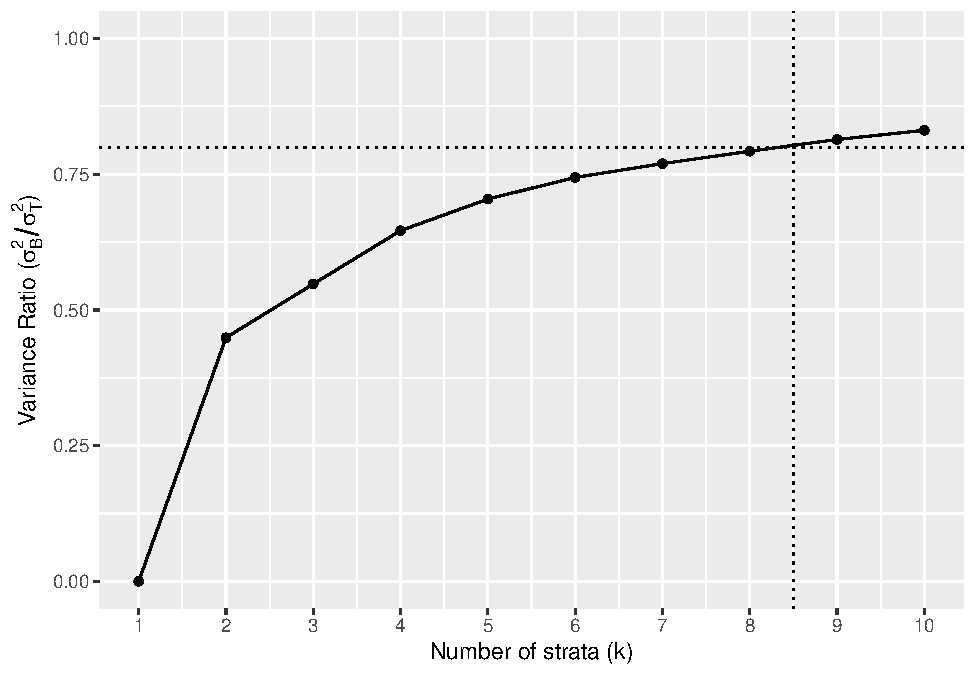
\includegraphics{5---Analysis_files/figure-latex/unnamed-chunk-4-1.pdf}

\hypertarget{methods-summary}{%
\section{Methods Summary}\label{methods-summary}}

\hypertarget{cluster-analysis}{%
\subsection{Cluster Analysis}\label{cluster-analysis}}

\hypertarget{selecting-k}{%
\subsubsection{Selecting k}\label{selecting-k}}

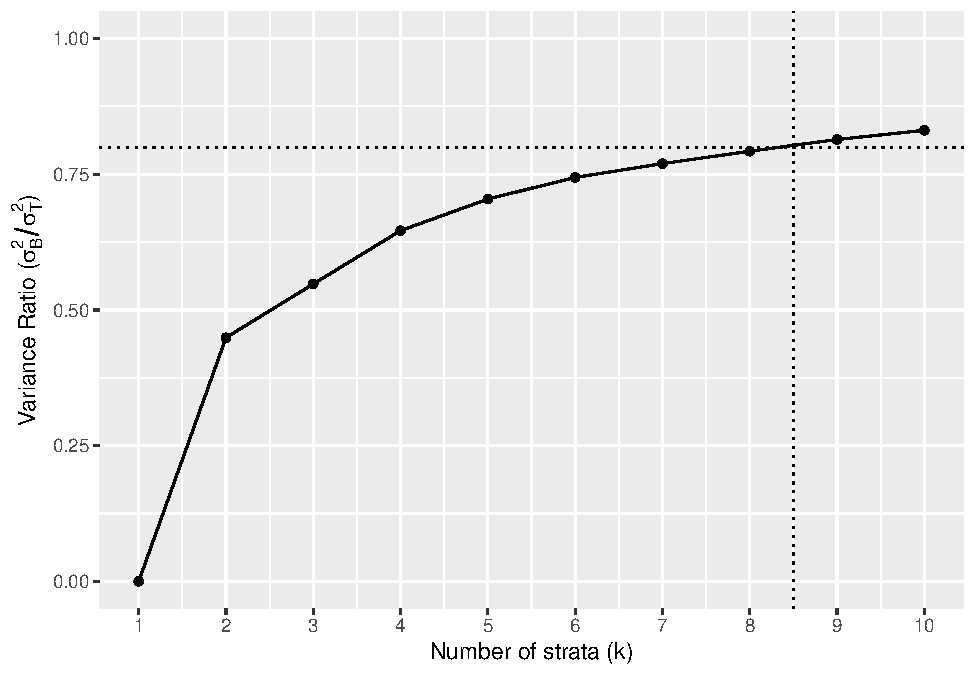
\includegraphics{5---Analysis_files/figure-latex/unnamed-chunk-5-1.pdf}

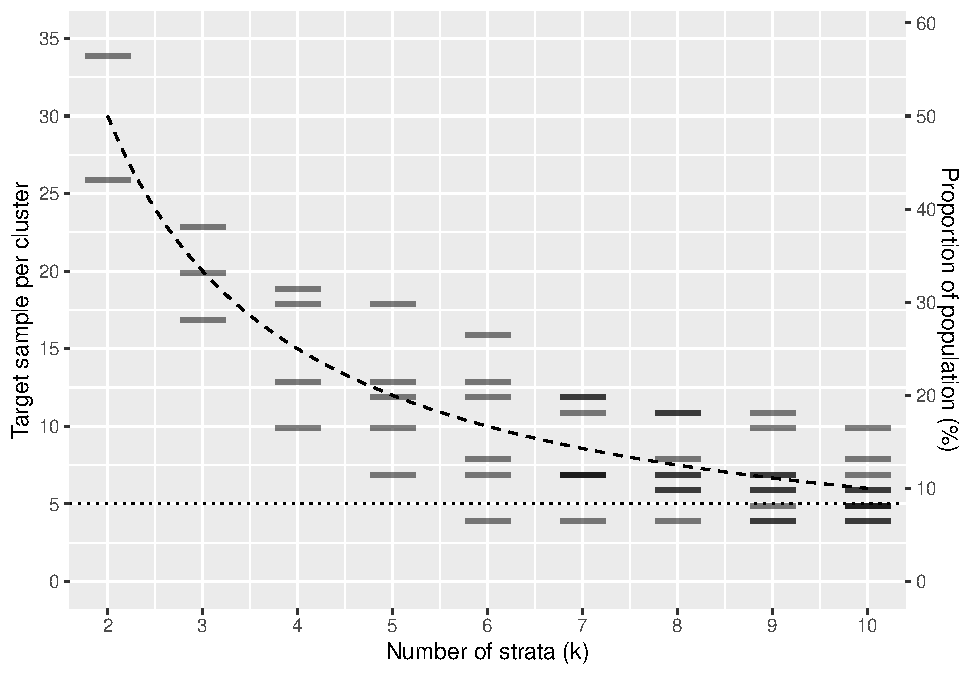
\includegraphics{5---Analysis_files/figure-latex/unnamed-chunk-6-1.pdf}

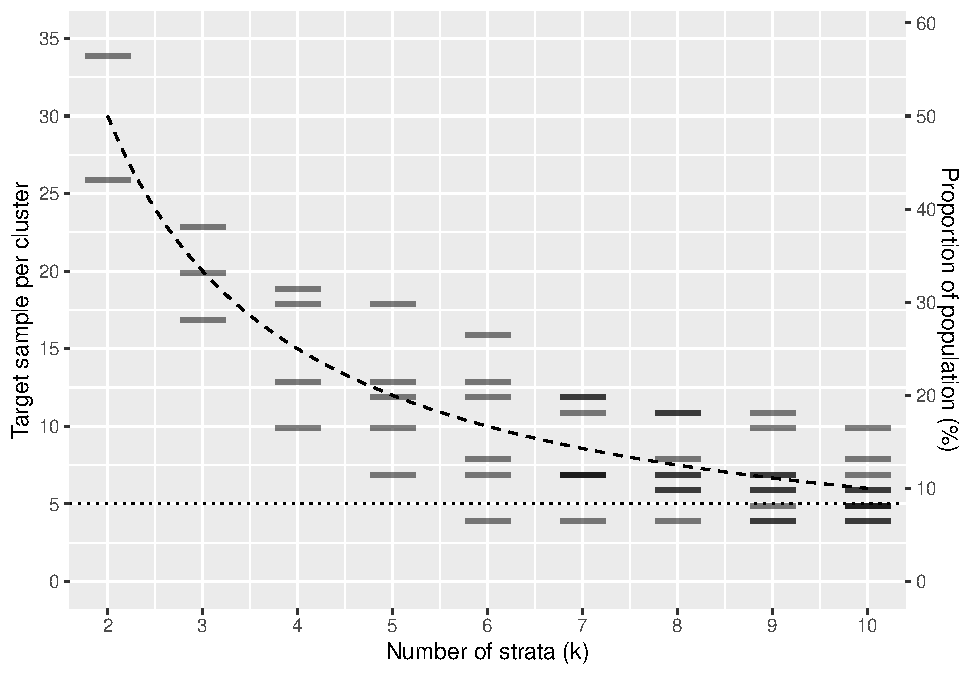
\includegraphics{5---Analysis_files/figure-latex/unnamed-chunk-7-1.pdf}

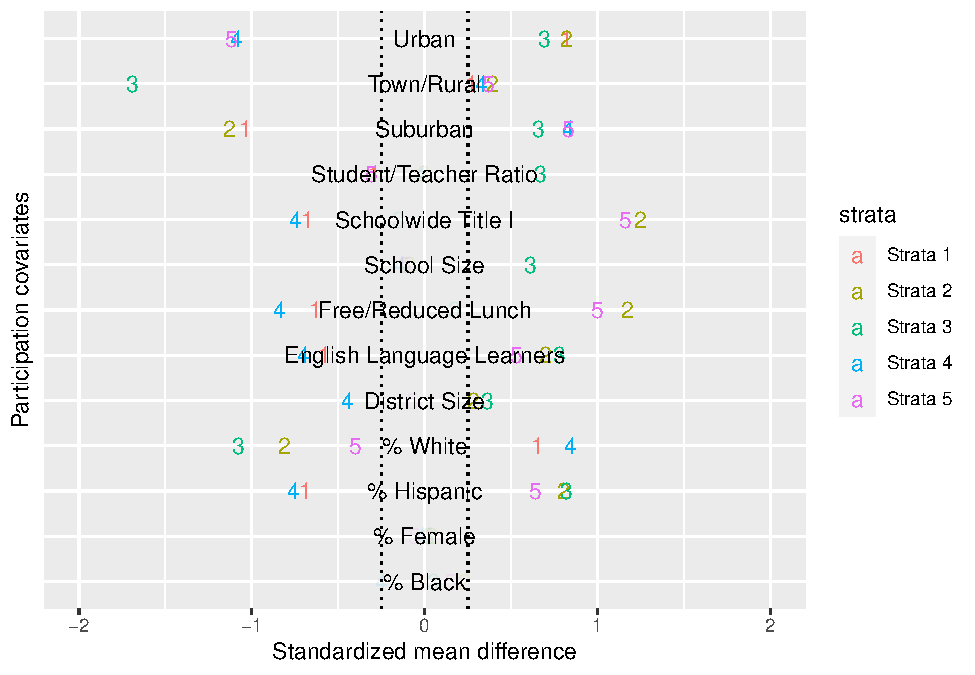
\includegraphics{5---Analysis_files/figure-latex/unnamed-chunk-8-1.pdf}

\begin{verbatim}
## Warning: Using alpha for a discrete variable is not advised.
\end{verbatim}

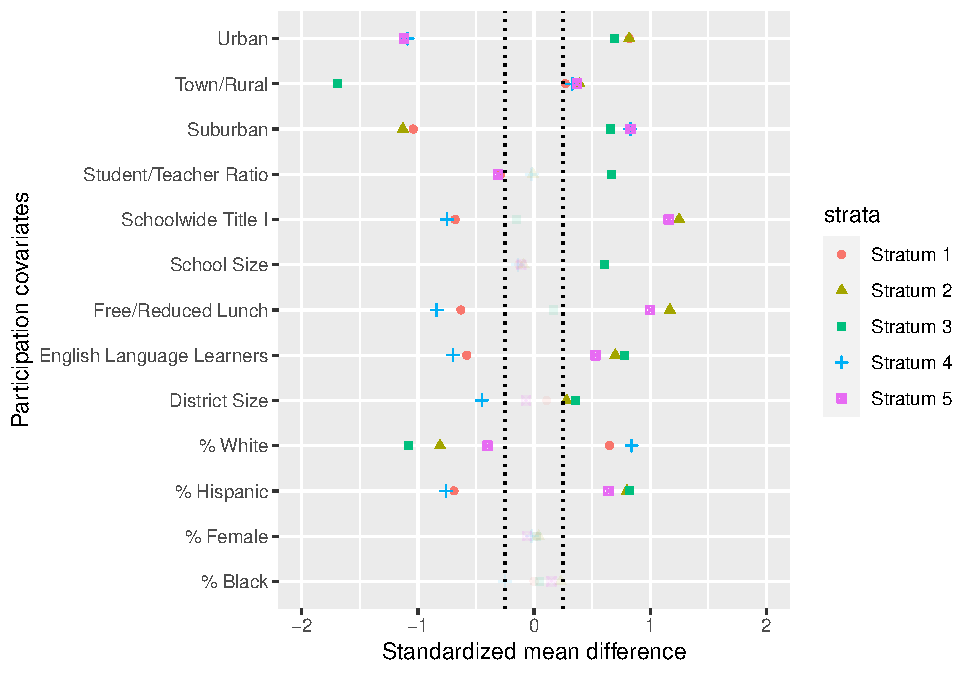
\includegraphics{5---Analysis_files/figure-latex/unnamed-chunk-10-1.pdf}

\hypertarget{variation-explained-by-the-strata}{%
\subsection{Variation explained by the strata}\label{variation-explained-by-the-strata}}

\hypertarget{participation-generating-model}{%
\subsection{Participation Generating Model}\label{participation-generating-model}}

\begin{table}
\centering
\begin{tabular}{l|l|l|l|r}
\hline
Sub & Category & Type & Variables & log\_odds\\
\hline
Status & School Data & Prop & Schoolwide Title I & 0.019\\
\hline
Enrollment & School Data & Mean & School Size & 0.374\\
\hline
Status & Student Data & Mean & Free/Reduced Lunch & 0.081\\
\hline
Urbanicity & School Data & Prop & Urban & 0.433\\
\hline
Urbanicity & School Data & Prop & Suburban & 0.007\\
\hline
Urbanicity & School Data & Prop & Town/Rural & -0.403\\
\hline
Ethnicity & Student Data & Mean & \% White & -0.538\\
\hline
Ethnicity & Student Data & Mean & \% Black & 0.291\\
\hline
Ethnicity & Student Data & Mean & \% Hispanic & 0.395\\
\hline
Gender & Student Data & Mean & \% Female & -0.019\\
\hline
Enrollment & School Data & Mean & Student/Teacher Ratio & -0.101\\
\hline
District & School Data & Mean & District Size & 0.520\\
\hline
Status & Student Data & Mean & English Language Learners & 0.412\\
\hline
\end{tabular}
\end{table}

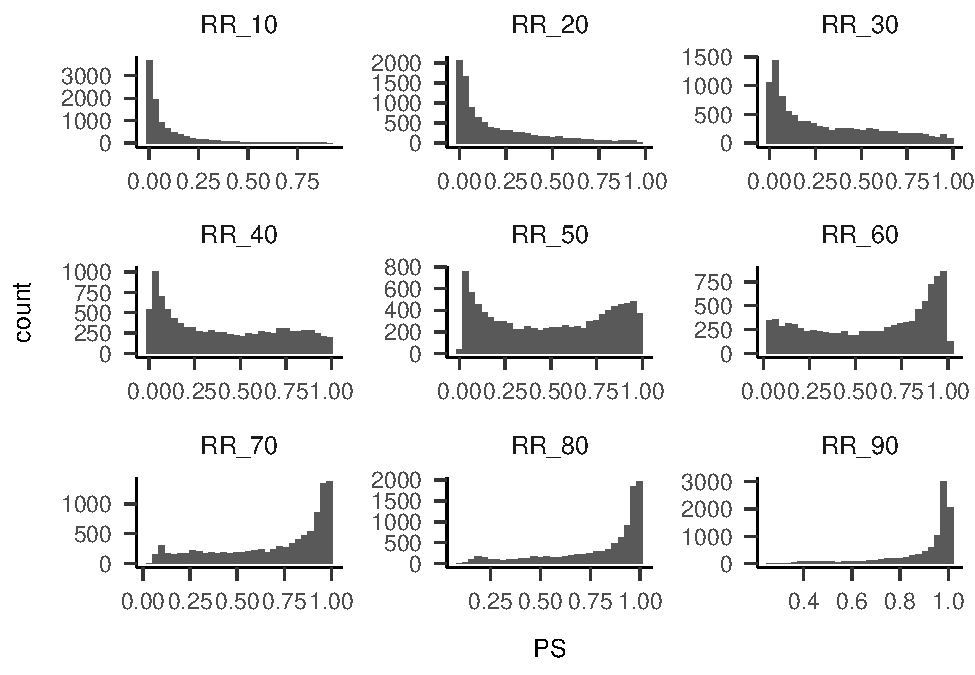
\includegraphics{5---Analysis_files/figure-latex/unnamed-chunk-13-1.pdf}

\begin{figure}
\centering
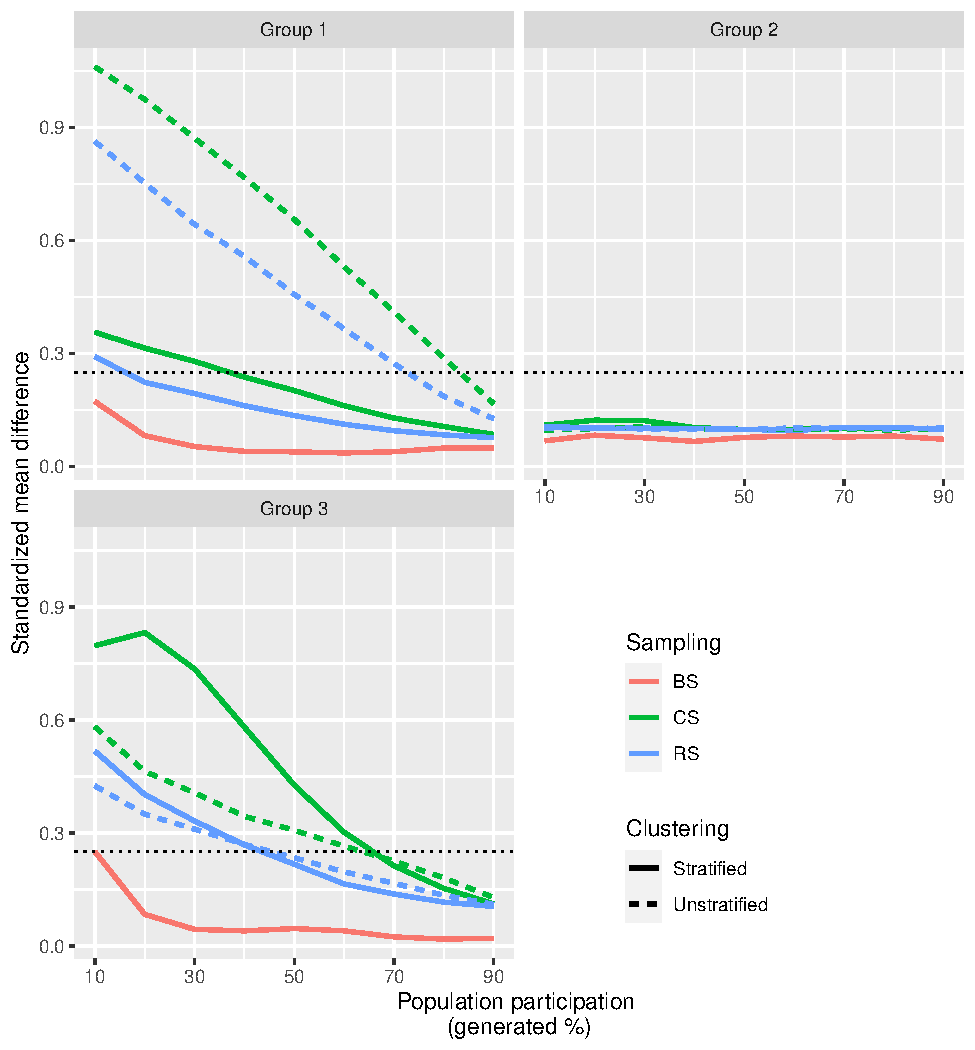
\includegraphics{5---Analysis_files/figure-latex/unnamed-chunk-14-1.pdf}
\caption{\label{fig:unnamed-chunk-14}Distributions of Participation Logits}
\end{figure}

\hypertarget{results}{%
\section{Results}\label{results}}

\hypertarget{generalizability}{%
\subsection{Generalizability}\label{generalizability}}

\hypertarget{b-index}{%
\subsubsection{B Index}\label{b-index}}

\begin{figure}
\centering
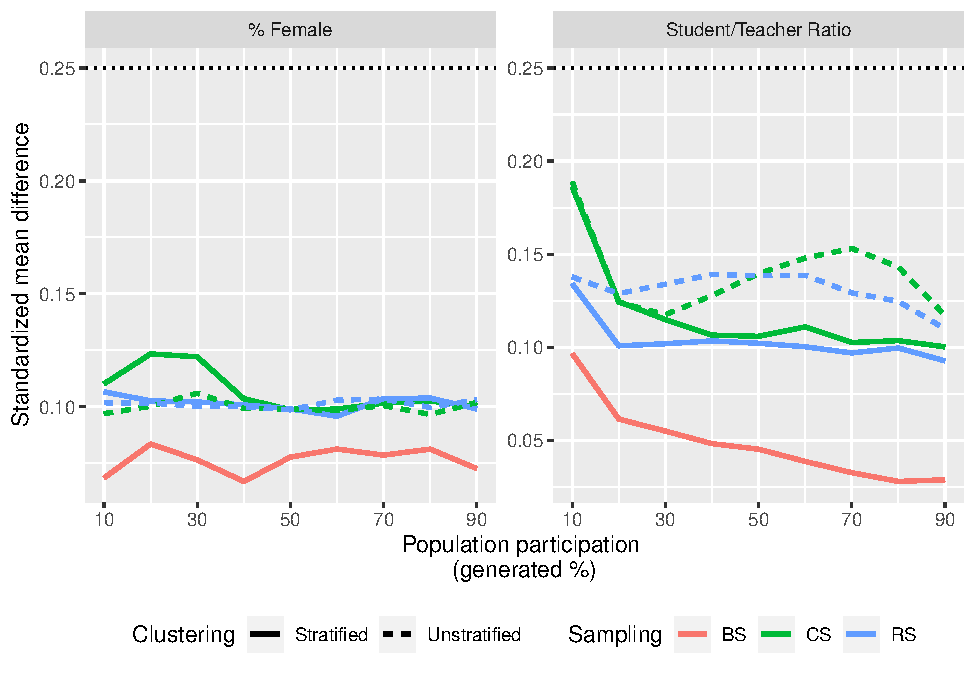
\includegraphics{5---Analysis_files/figure-latex/unnamed-chunk-16-1.pdf}
\caption{\label{fig:unnamed-chunk-16}Averge B-Index}
\end{figure}

\begin{verbatim}
## Note: Using an external vector in selections is ambiguous.
## i Use `all_of(variable)` instead of `variable` to silence this message.
## i See <https://tidyselect.r-lib.org/reference/faq-external-vector.html>.
## This message is displayed once per session.
## Note: Using an external vector in selections is ambiguous.
## i Use `all_of(observations)` instead of `observations` to silence this message.
## i See <https://tidyselect.r-lib.org/reference/faq-external-vector.html>.
## This message is displayed once per session.
\end{verbatim}

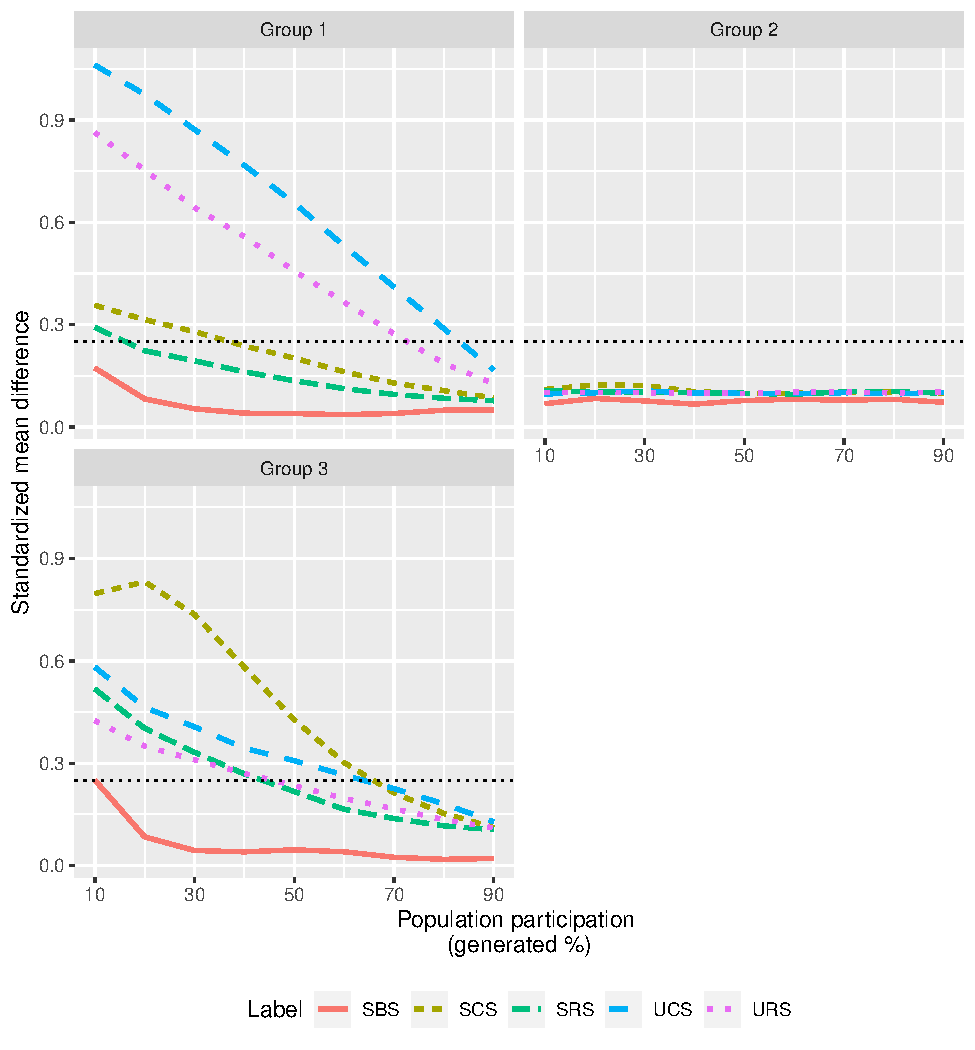
\includegraphics{5---Analysis_files/figure-latex/unnamed-chunk-17-1.pdf}

\hypertarget{smd}{%
\subsubsection{SMD}\label{smd}}

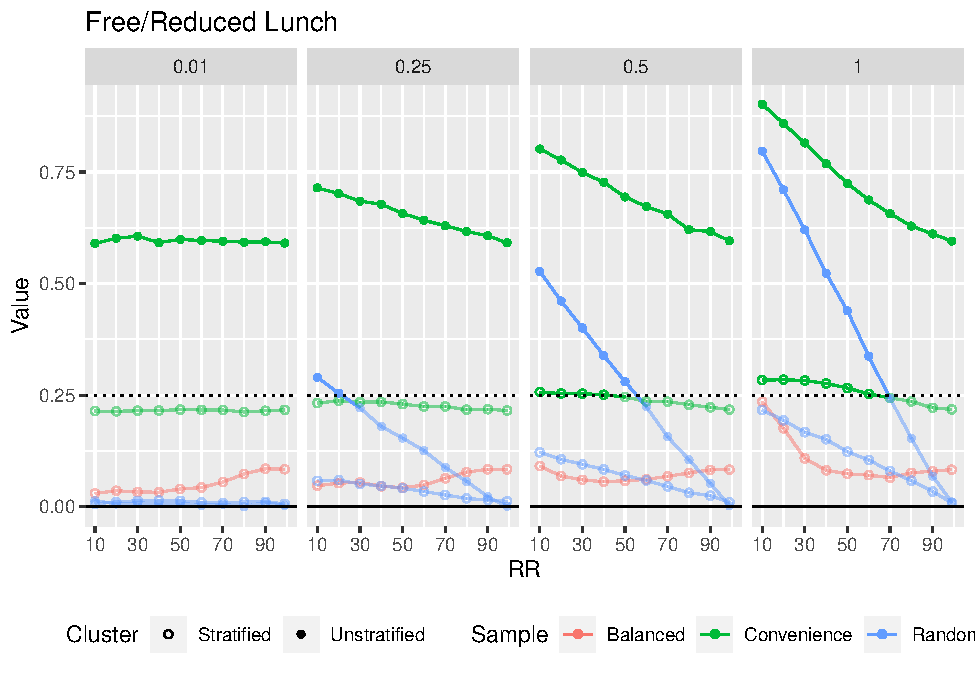
\includegraphics{5---Analysis_files/figure-latex/unnamed-chunk-19-1.pdf} 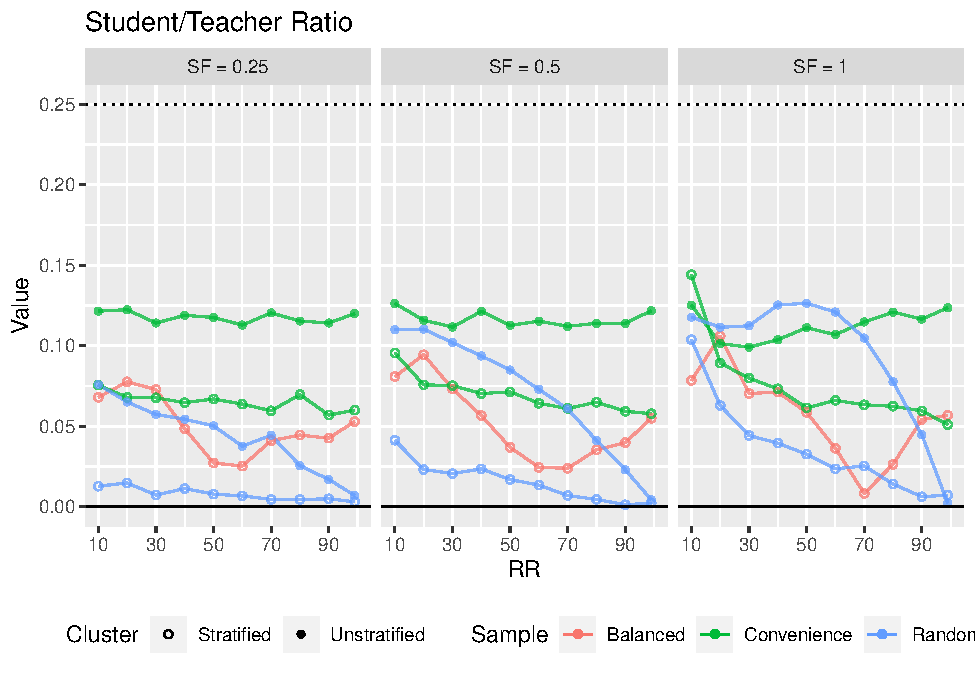
\includegraphics{5---Analysis_files/figure-latex/unnamed-chunk-19-2.pdf}

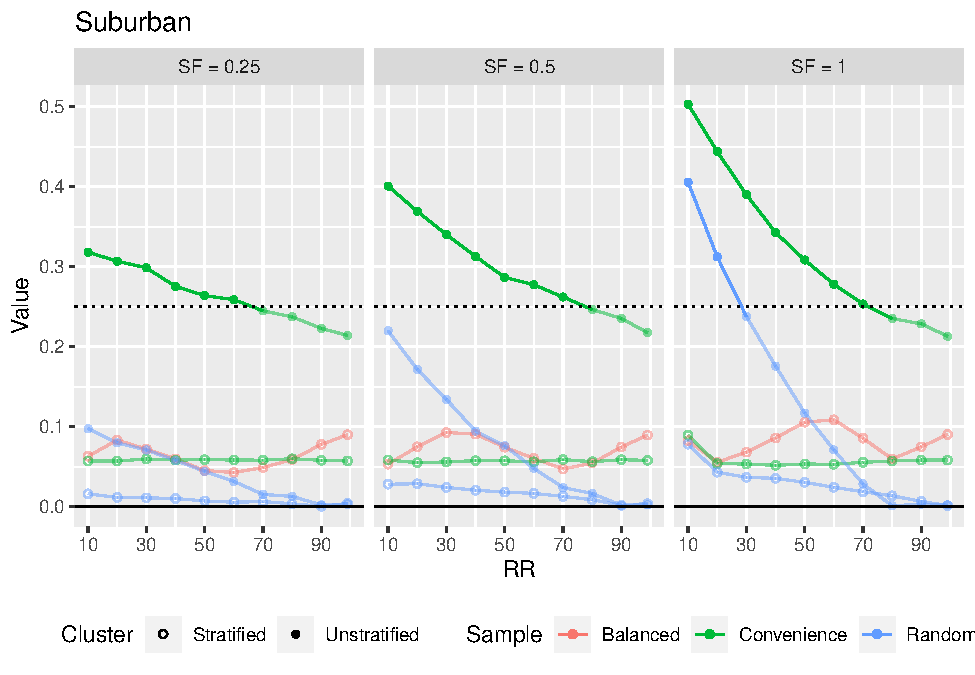
\includegraphics{5---Analysis_files/figure-latex/unnamed-chunk-20-1.pdf} 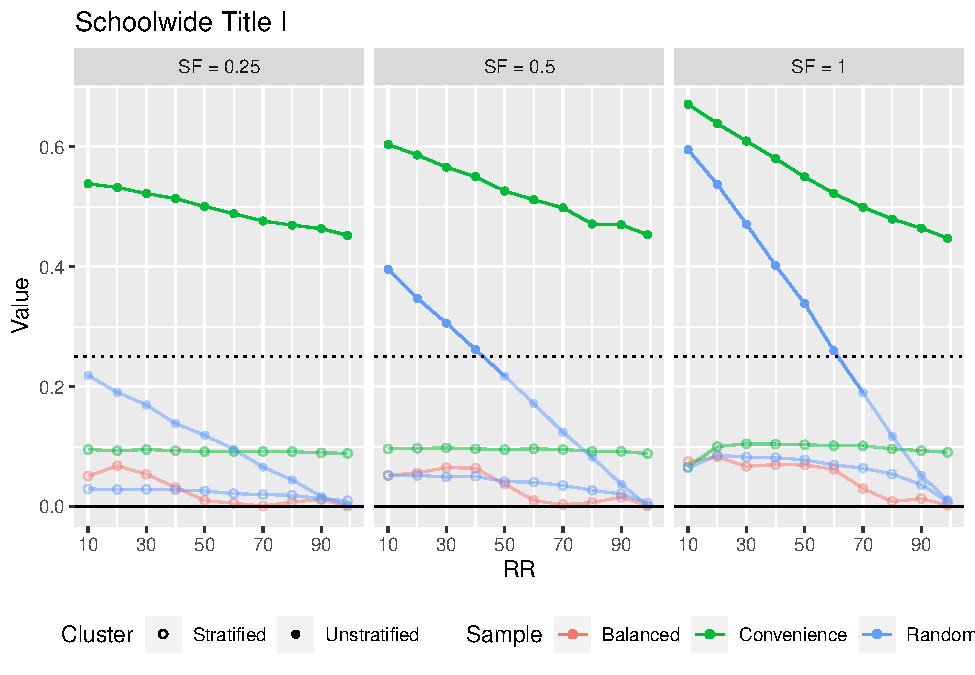
\includegraphics{5---Analysis_files/figure-latex/unnamed-chunk-20-2.pdf} 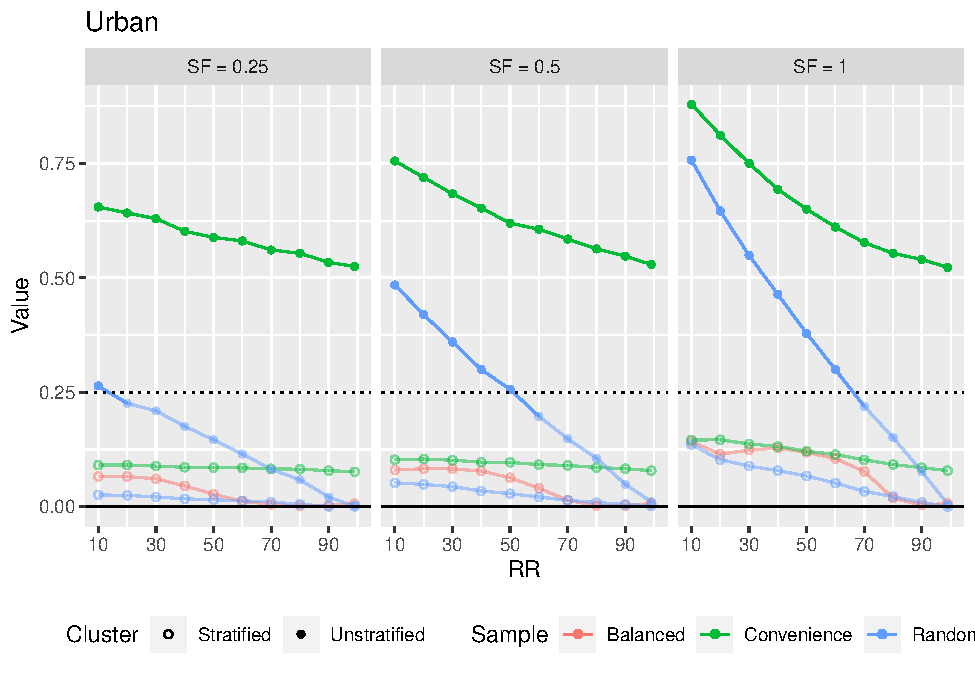
\includegraphics{5---Analysis_files/figure-latex/unnamed-chunk-20-3.pdf}

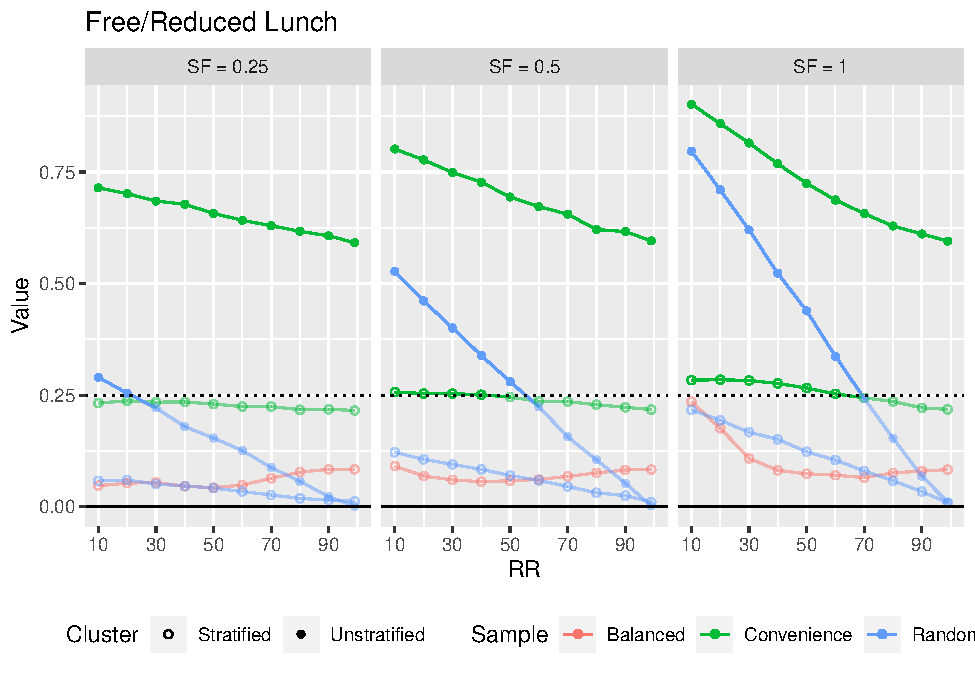
\includegraphics{5---Analysis_files/figure-latex/unnamed-chunk-21-1.pdf} 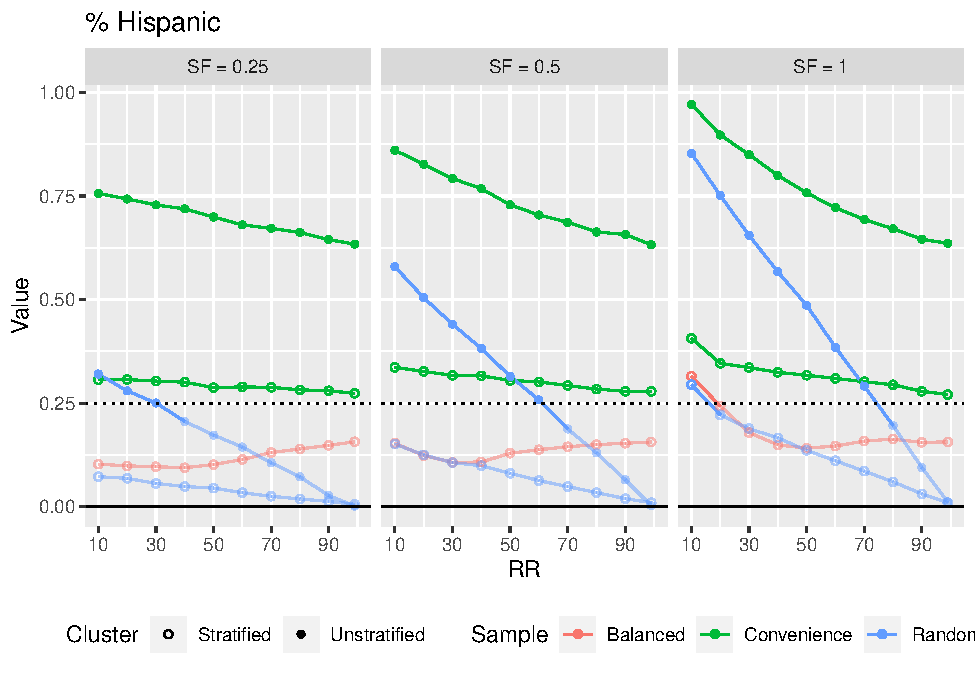
\includegraphics{5---Analysis_files/figure-latex/unnamed-chunk-21-2.pdf} 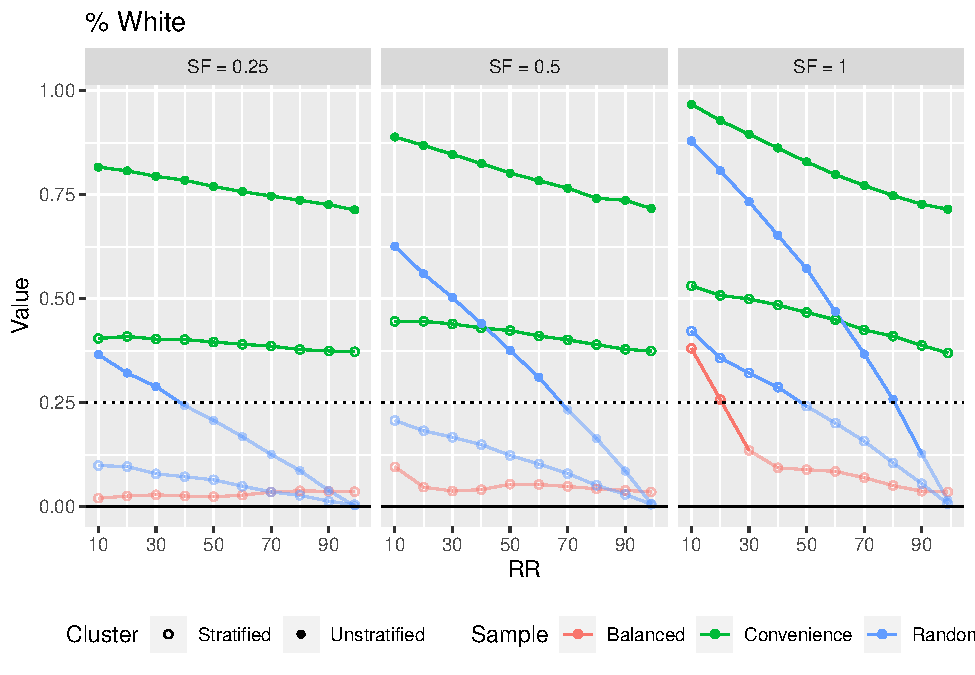
\includegraphics{5---Analysis_files/figure-latex/unnamed-chunk-21-3.pdf} 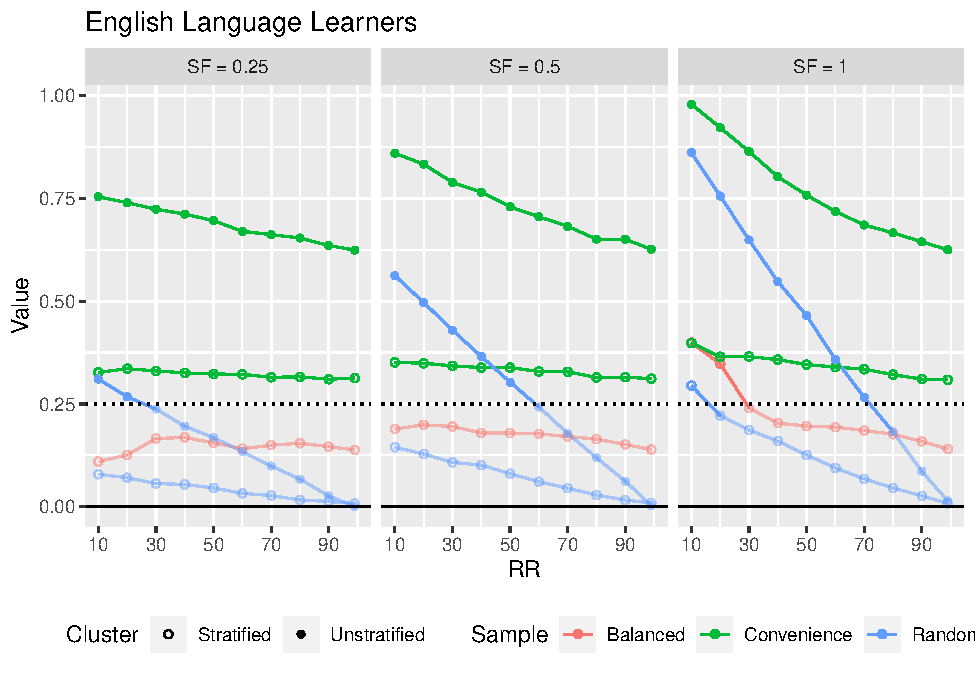
\includegraphics{5---Analysis_files/figure-latex/unnamed-chunk-21-4.pdf} 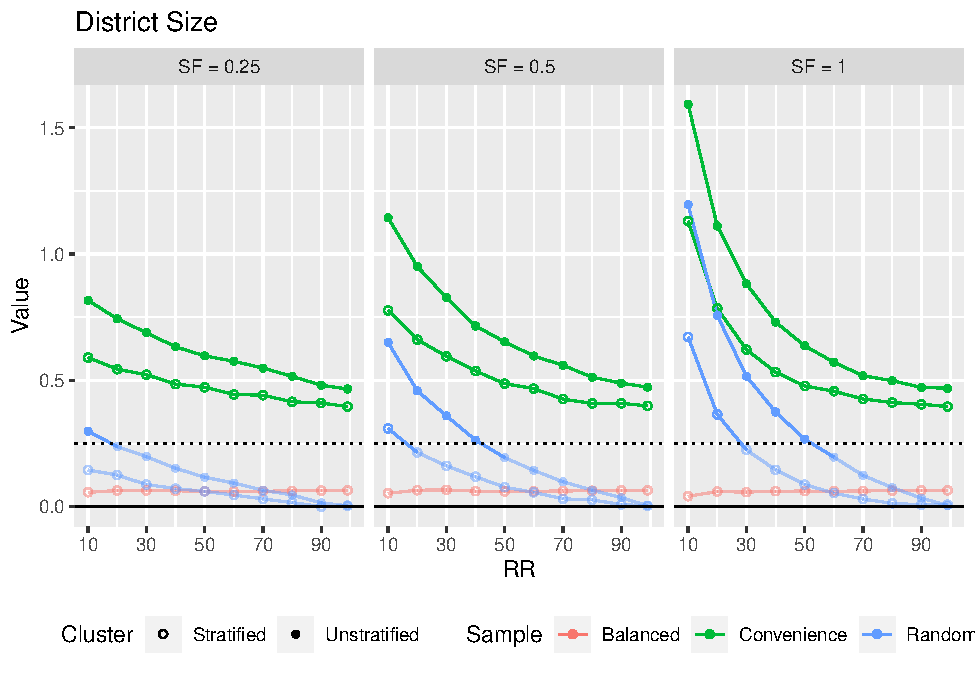
\includegraphics{5---Analysis_files/figure-latex/unnamed-chunk-21-5.pdf} 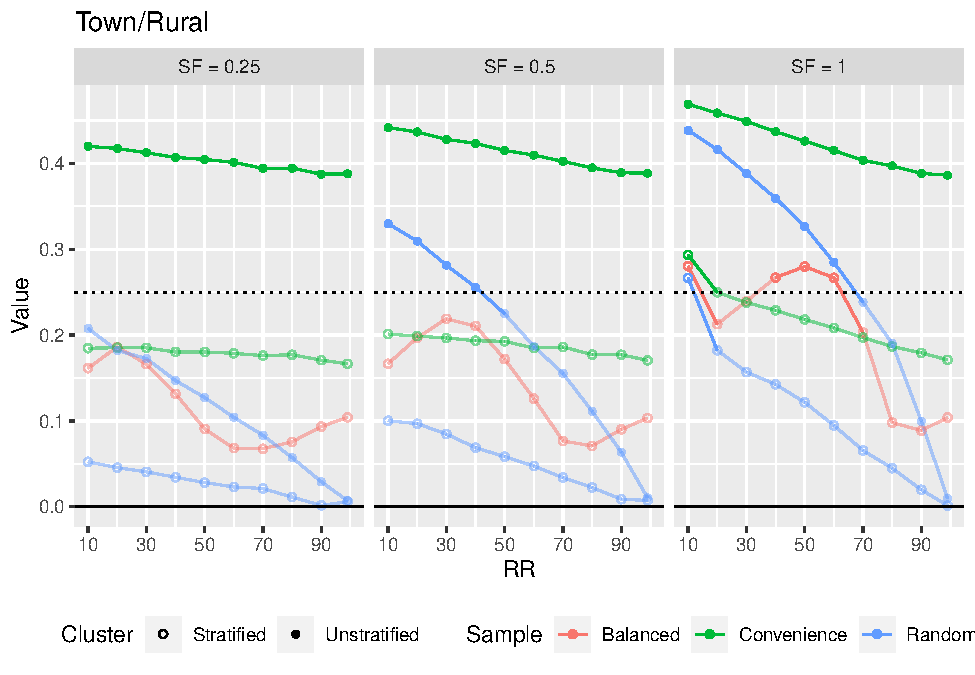
\includegraphics{5---Analysis_files/figure-latex/unnamed-chunk-21-6.pdf}

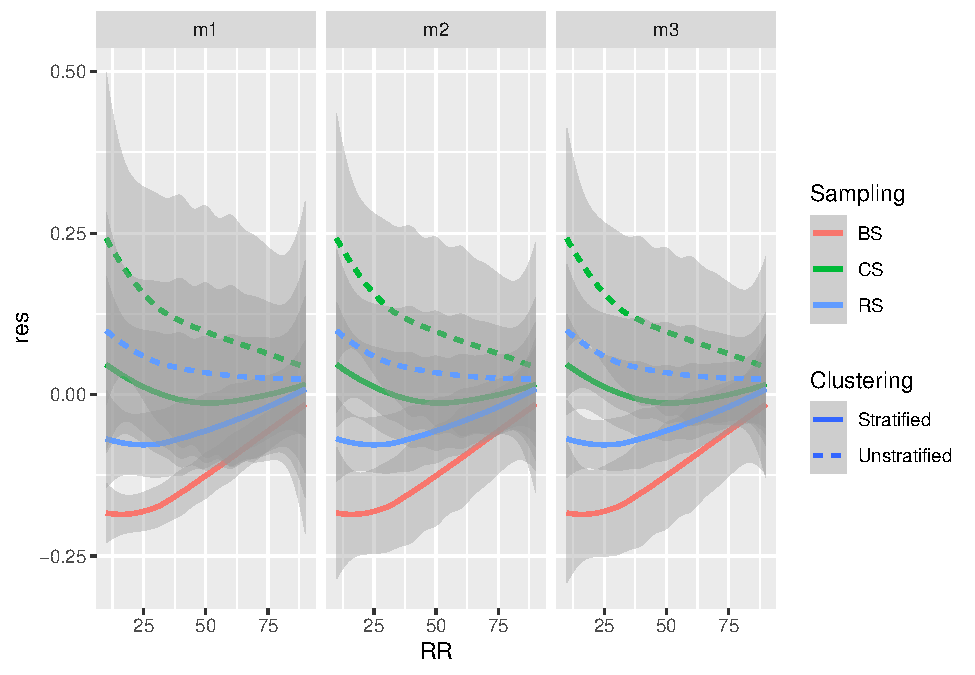
\includegraphics{5---Analysis_files/figure-latex/unnamed-chunk-22-1.pdf} 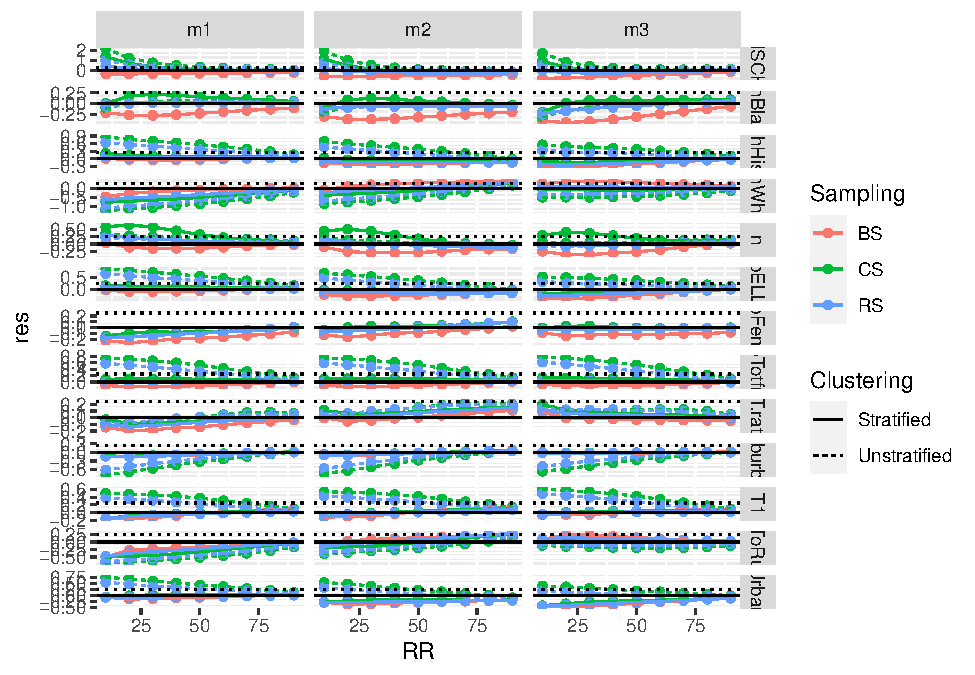
\includegraphics{5---Analysis_files/figure-latex/unnamed-chunk-22-2.pdf}

\hypertarget{smd-groups}{%
\subsubsection{SMD Groups}\label{smd-groups}}

\hypertarget{example-all-sf}{%
\paragraph{Example all SF}\label{example-all-sf}}

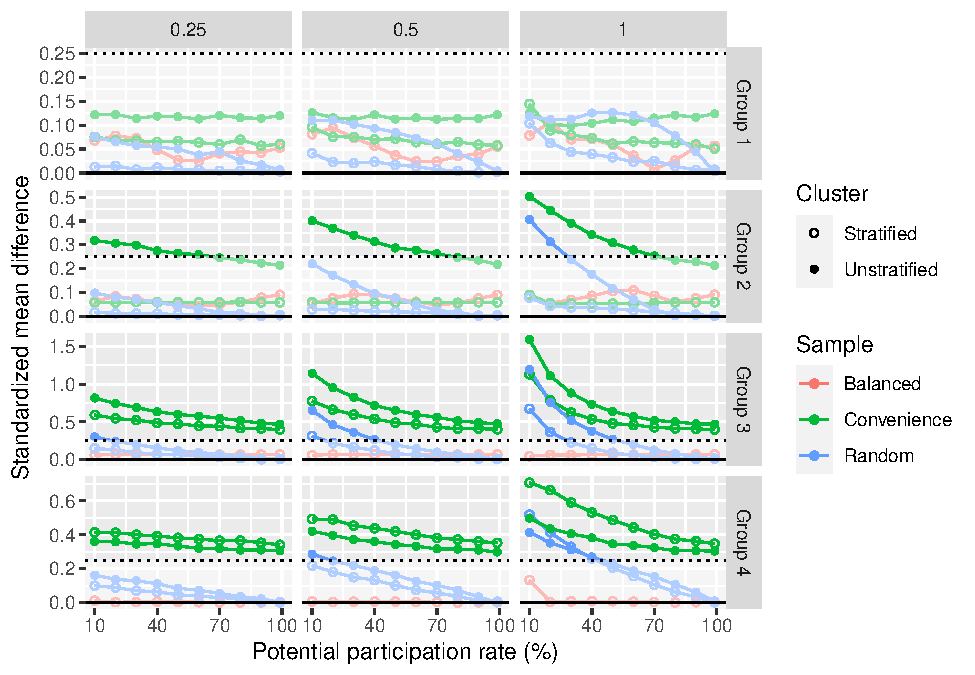
\includegraphics{5---Analysis_files/figure-latex/unnamed-chunk-24-1.pdf}

\hypertarget{example-sf-1}{%
\paragraph{Example SF = 1}\label{example-sf-1}}

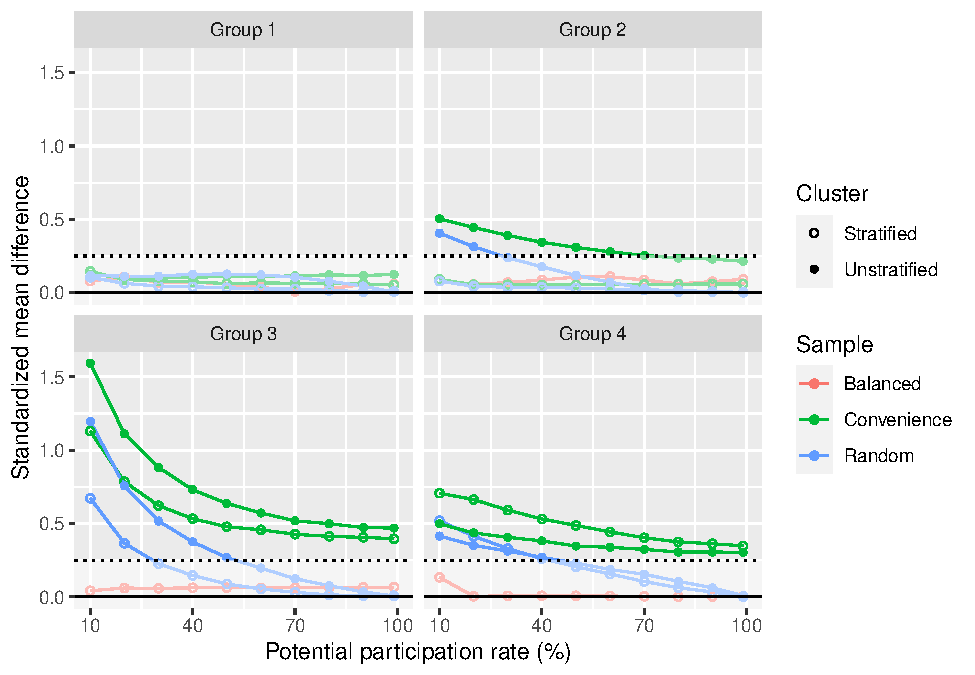
\includegraphics{5---Analysis_files/figure-latex/unnamed-chunk-25-1.pdf}

\hypertarget{auto-grouping}{%
\subsubsection{Auto-Grouping}\label{auto-grouping}}

\hypertarget{group-1}{%
\paragraph{Group 1}\label{group-1}}

\hypertarget{a-tibble-8-x-3}{%
\section{A tibble: 8 x 3}\label{a-tibble-8-x-3}}

\hypertarget{groups-sb-3}{%
\section{Groups: SB {[}3{]}}\label{groups-sb-3}}

\begin{verbatim}
 SB vnames   Group  
\end{verbatim}

\strut \\
1 0.25 ethBlack Group 1
2 0.5 ethBlack Group 1
3 0.25 pFem Group 1
4 0.5 pFem Group 1
5 1 pFem Group 1
6 0.25 ST.ratio Group 1
7 0.5 ST.ratio Group 1
8 1 ST.ratio Group 1

\$ethBlack
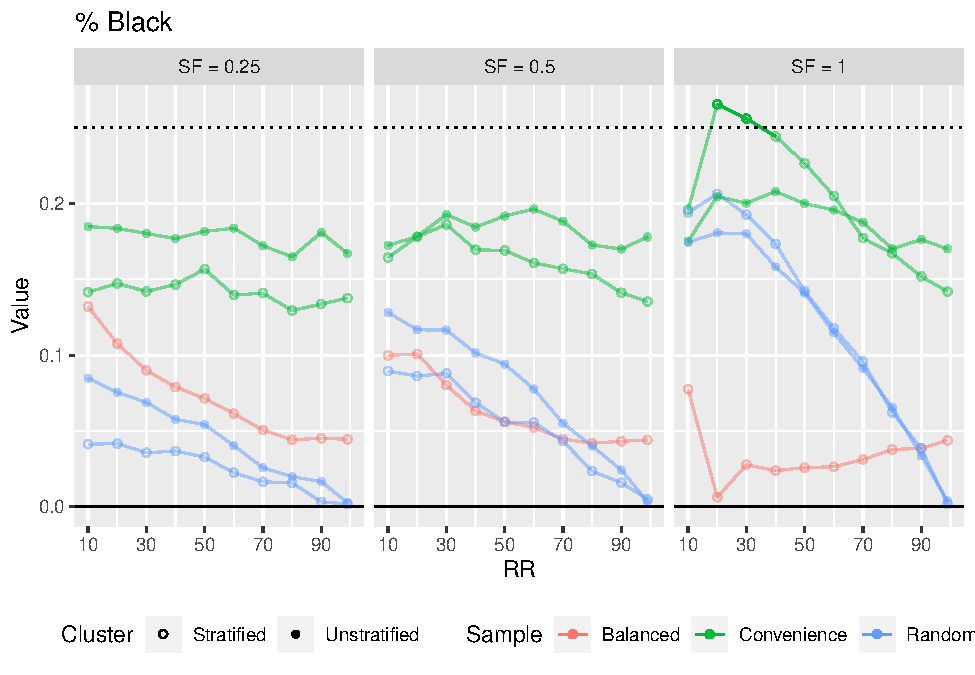
\includegraphics{5---Analysis_files/figure-latex/unnamed-chunk-28-1.pdf}
\$pFem
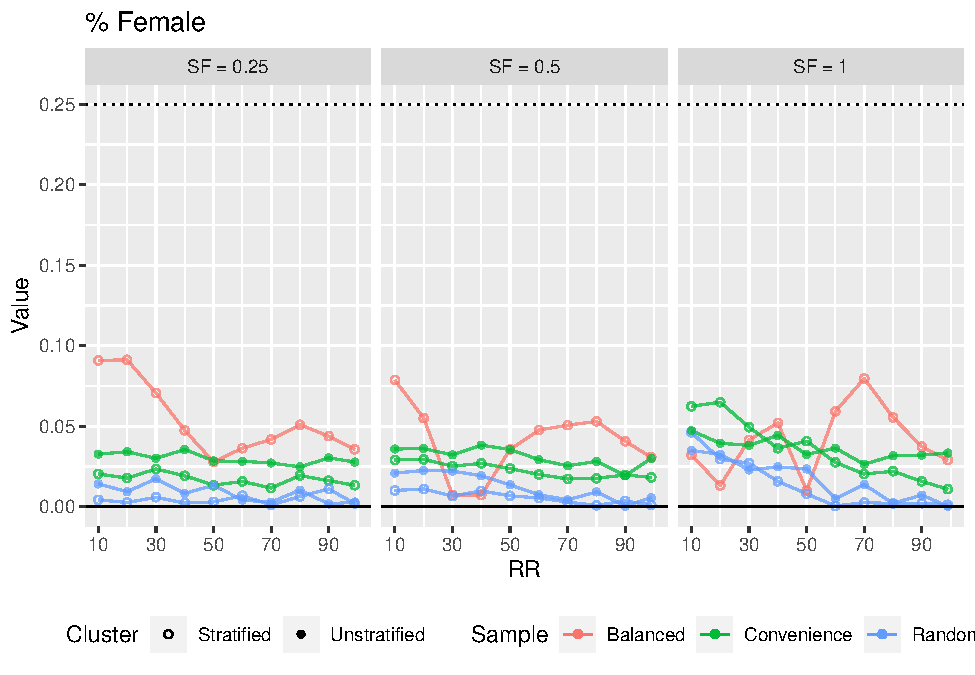
\includegraphics{5---Analysis_files/figure-latex/unnamed-chunk-28-2.pdf}
\$ST.ratio
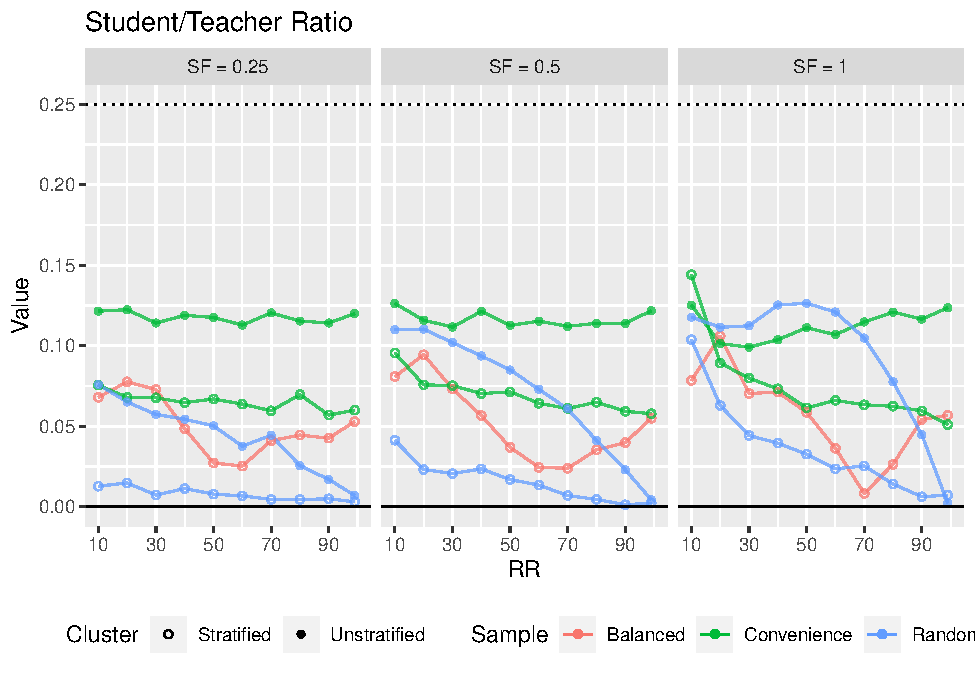
\includegraphics{5---Analysis_files/figure-latex/unnamed-chunk-28-3.pdf}

\hypertarget{group-2}{%
\paragraph{Group 2}\label{group-2}}

\hypertarget{a-tibble-12-x-3}{%
\section{A tibble: 12 x 3}\label{a-tibble-12-x-3}}

\begin{verbatim}
  SB vnames   Group  
\end{verbatim}

\strut \\
1 0.25 pTotfrl Group 2
2 0.25 Suburban Group 2
3 0.5 Suburban Group 2
4 1 Suburban Group 2
5 0.25 T1 Group 2
6 0.5 T1 Group 2
7 1 T1 Group 2
8 0.25 ToRu Group 2
9 0.5 ToRu Group 2
10 0.25 Urban Group 2
11 0.5 Urban Group 2
12 1 Urban Group 2

\$pTotfrl
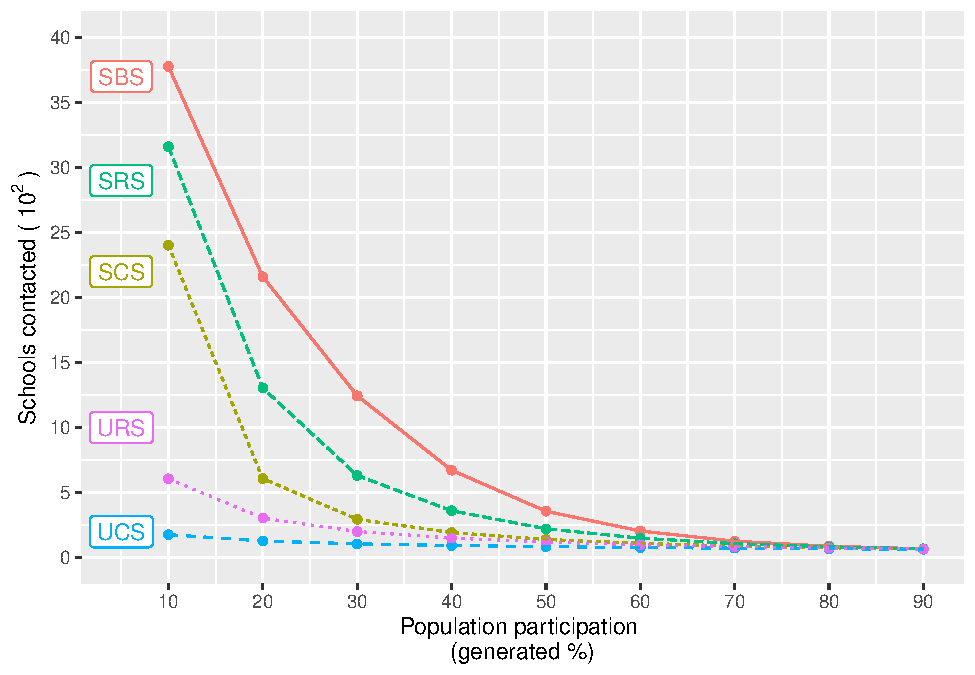
\includegraphics{5---Analysis_files/figure-latex/unnamed-chunk-30-1.pdf}
\$Suburban
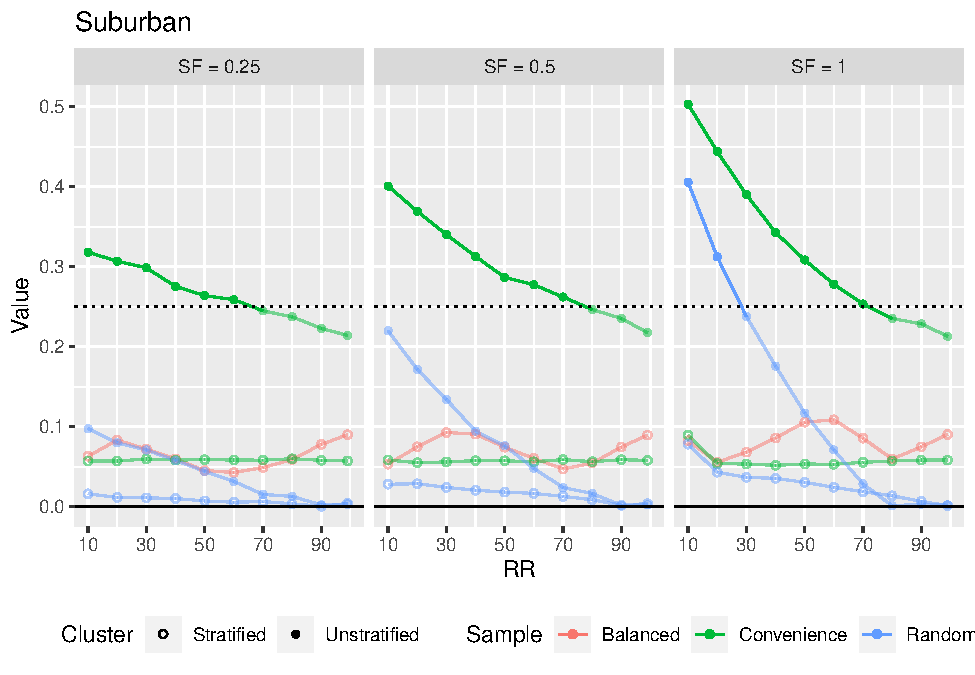
\includegraphics{5---Analysis_files/figure-latex/unnamed-chunk-30-2.pdf}
\$T1
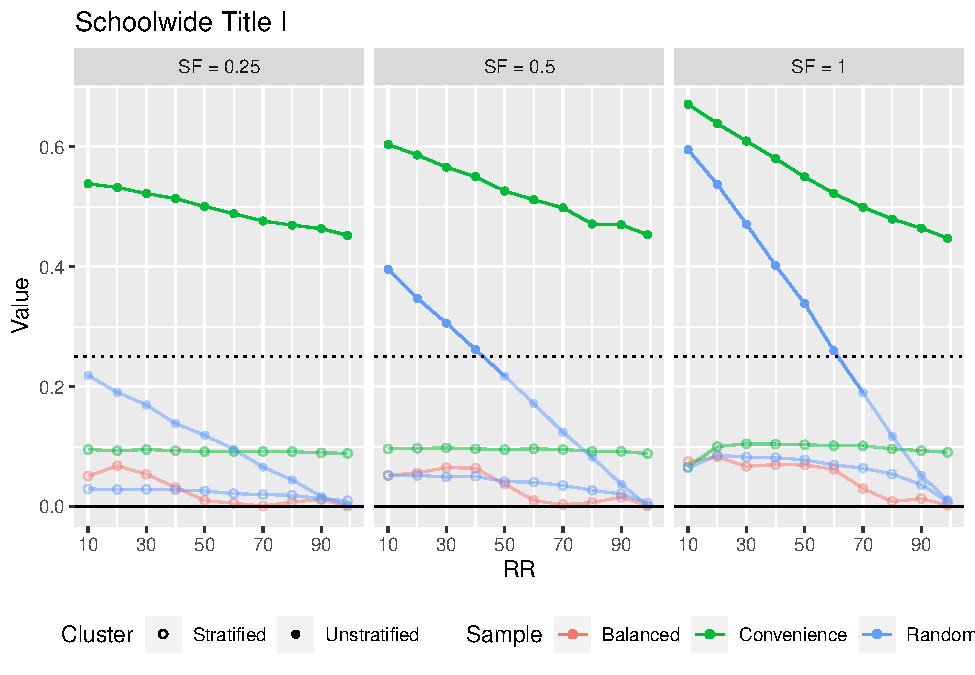
\includegraphics{5---Analysis_files/figure-latex/unnamed-chunk-30-3.pdf}
\$ToRu
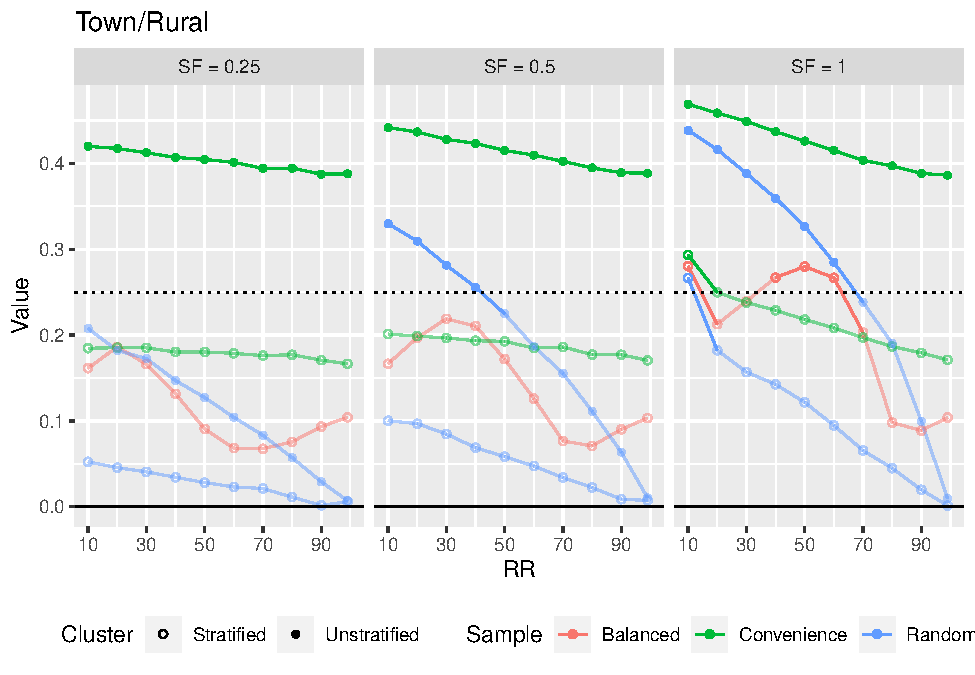
\includegraphics{5---Analysis_files/figure-latex/unnamed-chunk-30-4.pdf}
\$Urban
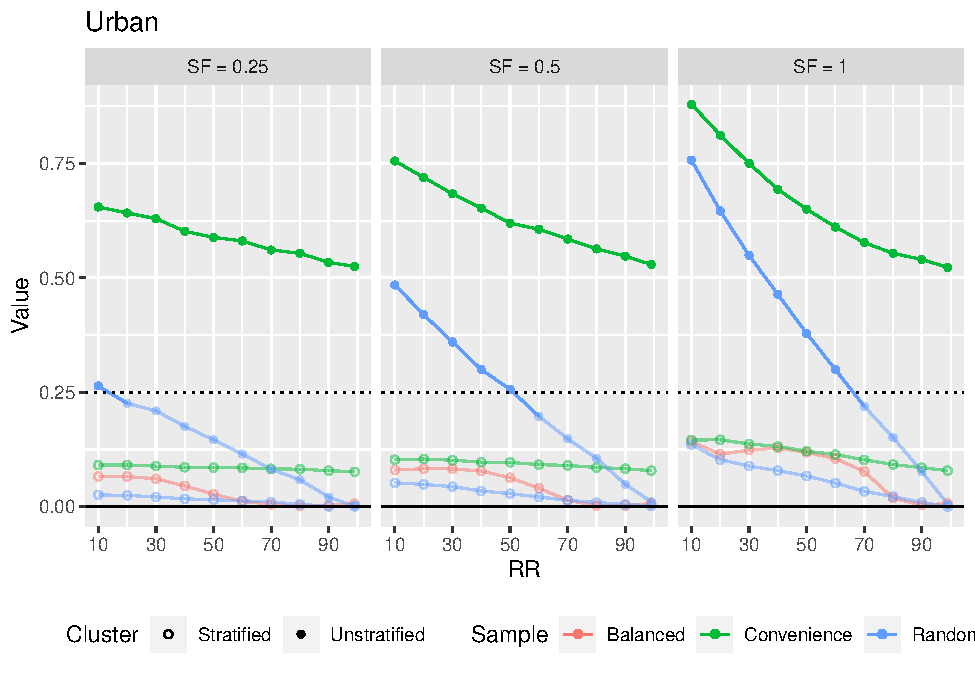
\includegraphics{5---Analysis_files/figure-latex/unnamed-chunk-30-5.pdf}

\hypertarget{group-3}{%
\paragraph{Group 3}\label{group-3}}

\hypertarget{a-tibble-15-x-3}{%
\section{A tibble: 15 x 3}\label{a-tibble-15-x-3}}

\begin{verbatim}
  SB vnames   Group  
\end{verbatim}

\strut \\
1 0.25 dSCH Group 3
2 0.5 dSCH Group 3
3 1 dSCH Group 3
4 0.25 ethHisp Group 3
5 0.5 ethHisp Group 3
6 1 ethHisp Group 3
7 0.25 ethWhite Group 3
8 0.5 ethWhite Group 3
9 1 ethWhite Group 3
10 0.25 pELL Group 3
11 0.5 pELL Group 3
12 1 pELL Group 3
13 0.5 pTotfrl Group 3
14 1 pTotfrl Group 3
15 1 ToRu Group 3

\$pTotfrl
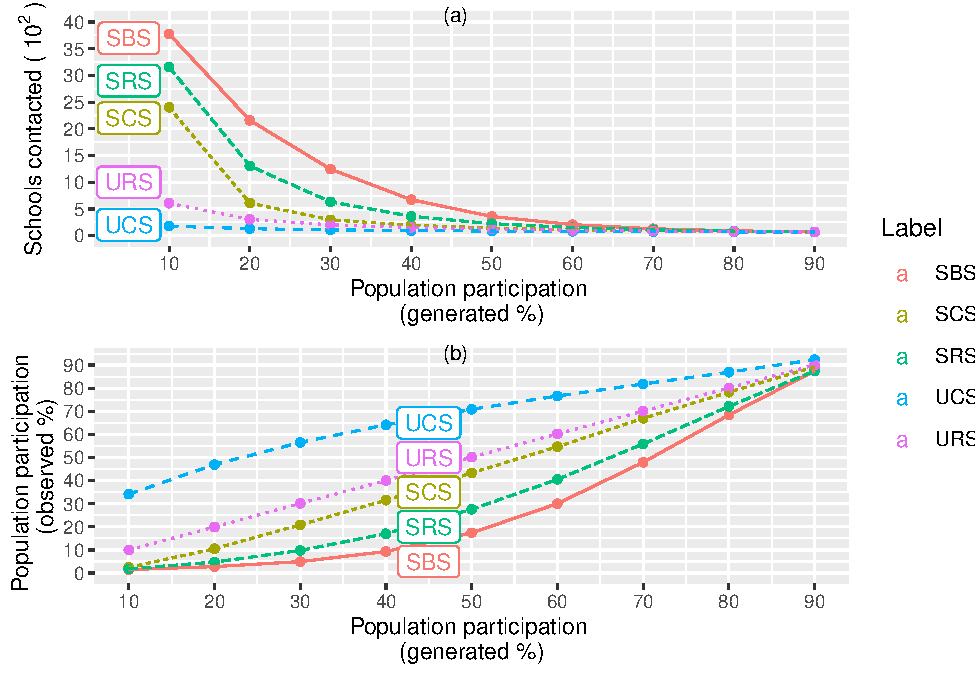
\includegraphics{5---Analysis_files/figure-latex/unnamed-chunk-32-1.pdf}
\$Suburban
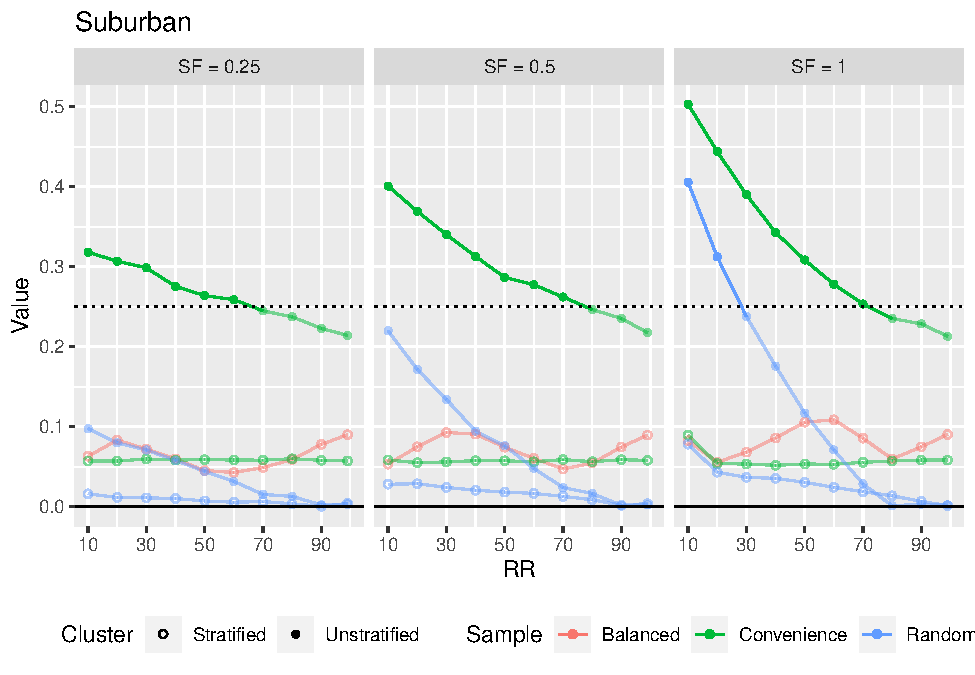
\includegraphics{5---Analysis_files/figure-latex/unnamed-chunk-32-2.pdf}
\$T1
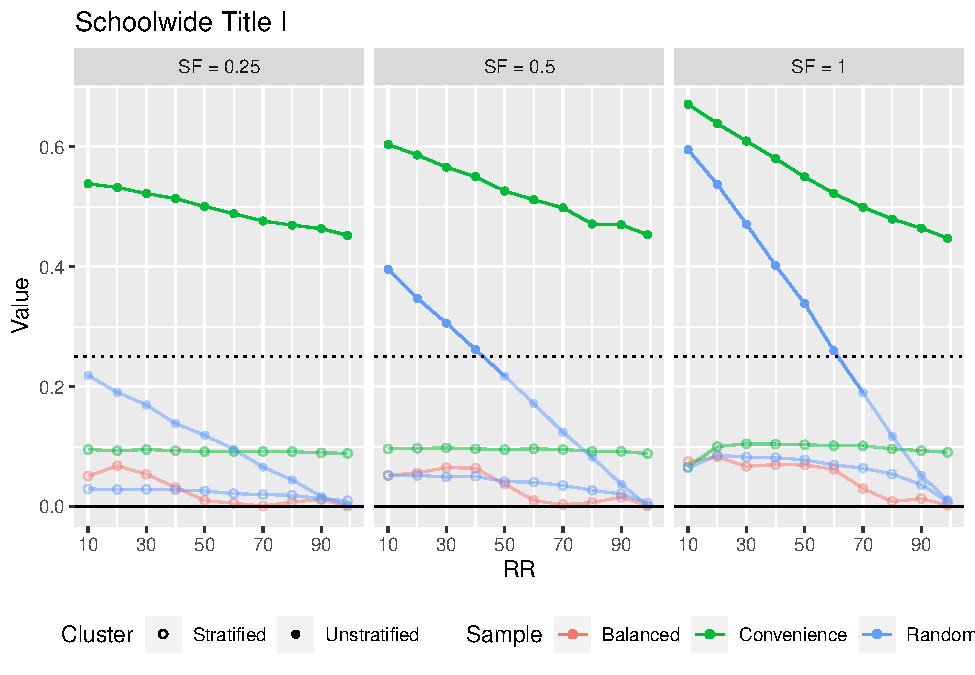
\includegraphics{5---Analysis_files/figure-latex/unnamed-chunk-32-3.pdf}
\$ToRu
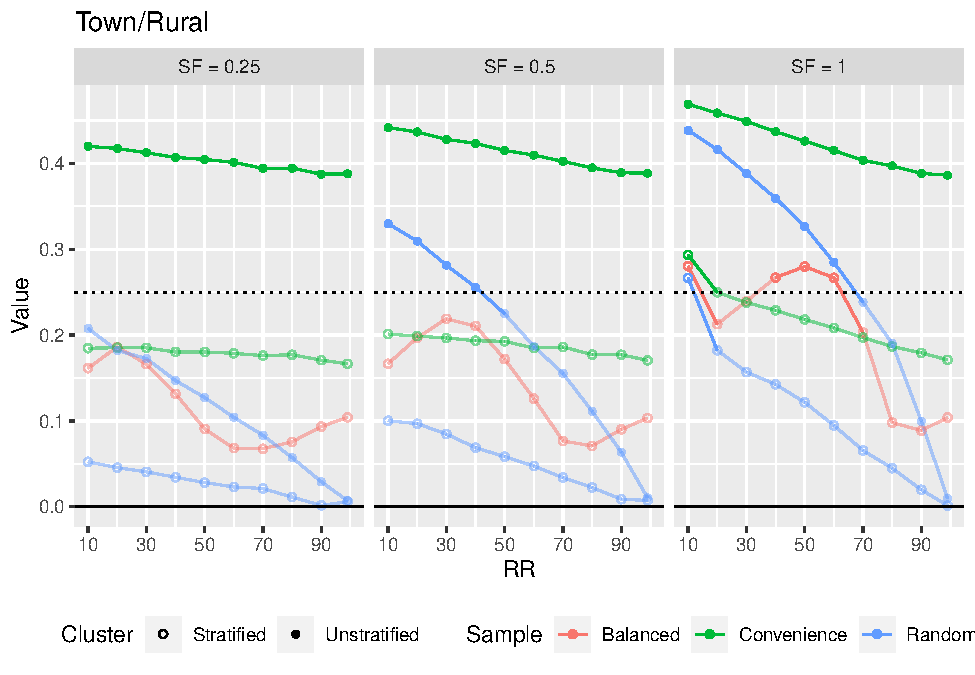
\includegraphics{5---Analysis_files/figure-latex/unnamed-chunk-32-4.pdf}
\$Urban
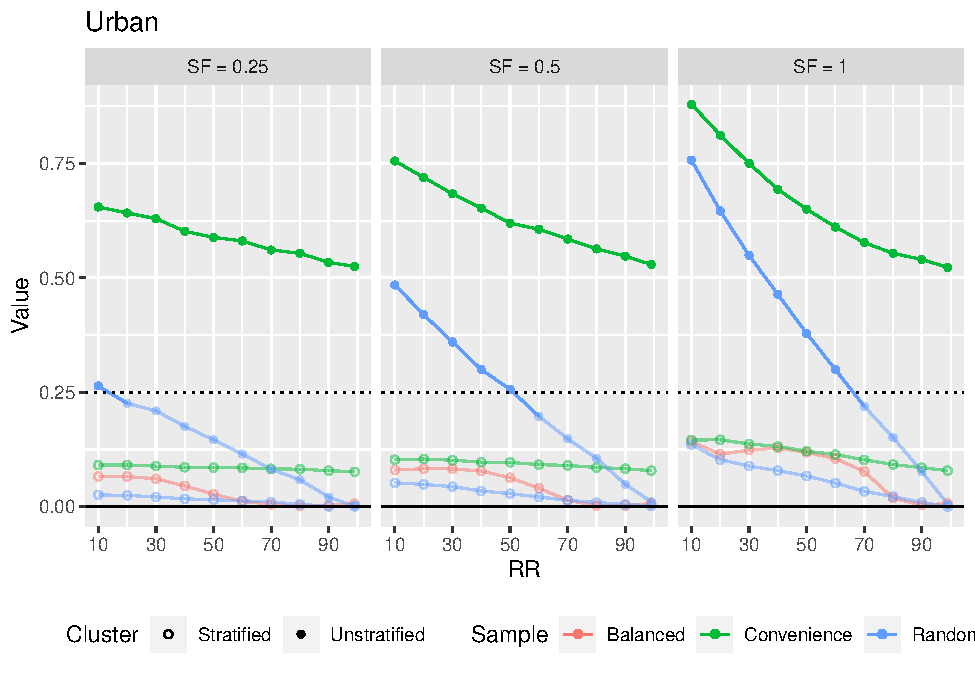
\includegraphics{5---Analysis_files/figure-latex/unnamed-chunk-32-5.pdf}
\#\#\#\# Group 4
\# A tibble: 4 x 3
SB vnames Group\\
\strut \\
1 1 ethBlack Group 4
2 0.25 n Group 4
3 0.5 n Group 4
4 1 n Group 4

\$ethBlack
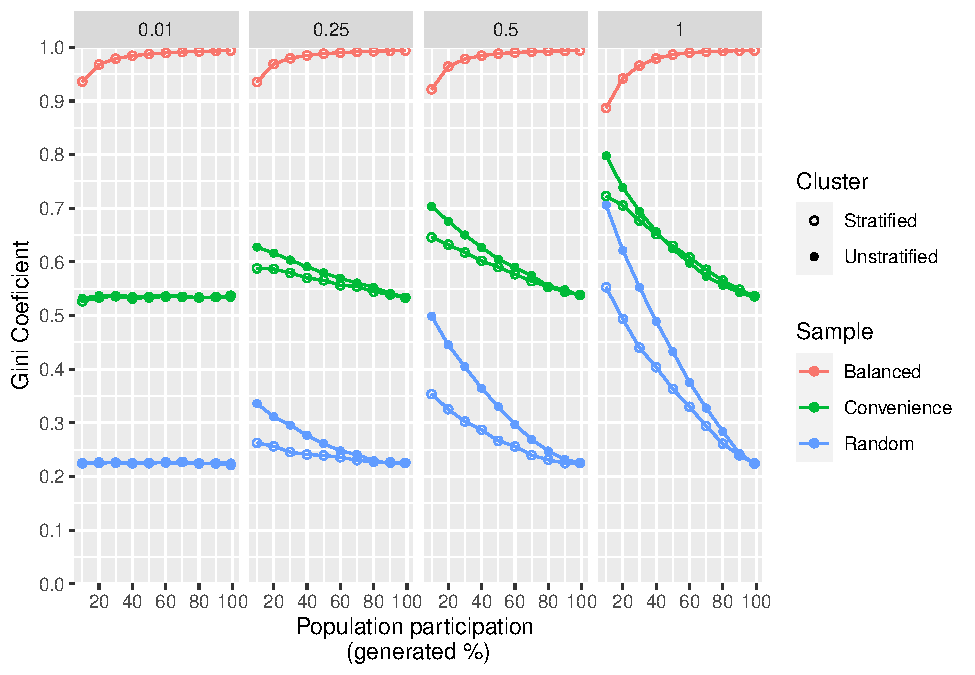
\includegraphics{5---Analysis_files/figure-latex/unnamed-chunk-34-1.pdf}
\$n
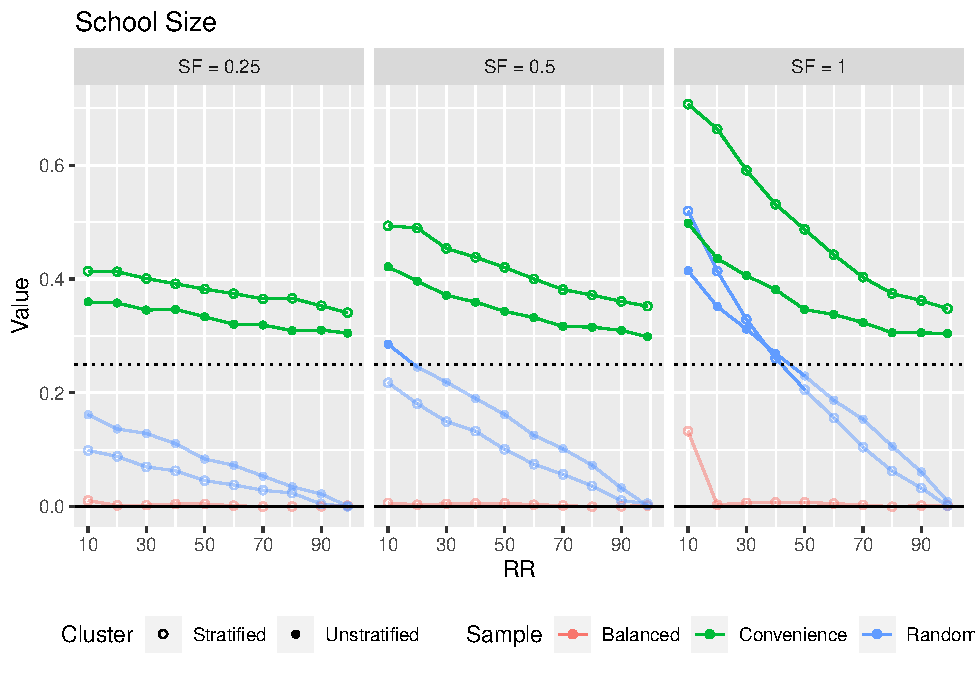
\includegraphics{5---Analysis_files/figure-latex/unnamed-chunk-34-2.pdf}

\hypertarget{fine-grain-groups}{%
\paragraph{Fine Grain Groups}\label{fine-grain-groups}}

\hypertarget{v-ratio-and-log-odds}{%
\subsubsection{V-ratio and Log odds}\label{v-ratio-and-log-odds}}

\hypertarget{a-tibble-39-x-15}{%
\section{A tibble: 39 x 15}\label{a-tibble-39-x-15}}

vnames T.SS W.SS B.SS vratio Sub Category Type Variables log\_odds
1 dSCH 4.02e8 3.62e8 4.05e7 0.101 Dist\textasciitilde{} School \textasciitilde{} Mean District\textasciitilde{} 0.52
2 dSCH 4.02e8 3.62e8 4.05e7 0.101 Dist\textasciitilde{} School \textasciitilde{} Mean District\textasciitilde{} 0.52
3 dSCH 4.02e8 3.62e8 4.05e7 0.101 Dist\textasciitilde{} School \textasciitilde{} Mean District\textasciitilde{} 0.52
4 ethBlack 2.52e6 2.44e6 7.96e4 0.0316 Ethn\textasciitilde{} Student\textasciitilde{} Mean \% Black 0.291
5 ethBlack 2.52e6 2.44e6 7.96e4 0.0316 Ethn\textasciitilde{} Student\textasciitilde{} Mean \% Black 0.291
6 ethBlack 2.52e6 2.44e6 7.96e4 0.0316 Ethn\textasciitilde{} Student\textasciitilde{} Mean \% Black 0.291
7 ethHisp 1.05e7 4.63e6 5.89e6 0.560 Ethn\textasciitilde{} Student\textasciitilde{} Mean \% Hispan\textasciitilde{} 0.395
8 ethHisp 1.05e7 4.63e6 5.89e6 0.560 Ethn\textasciitilde{} Student\textasciitilde{} Mean \% Hispan\textasciitilde{} 0.395
9 ethHisp 1.05e7 4.63e6 5.89e6 0.560 Ethn\textasciitilde{} Student\textasciitilde{} Mean \% Hispan\textasciitilde{} 0.395
10 ethWhite 9.10e6 3.28e6 5.83e6 0.640 Ethn\textasciitilde{} Student\textasciitilde{} Mean \% White -0.538
\# \ldots{} with 29 more rows, and 5 more variables: SB , Coeficient ,
\# abs\_log\_odds , SF\_fac , Group

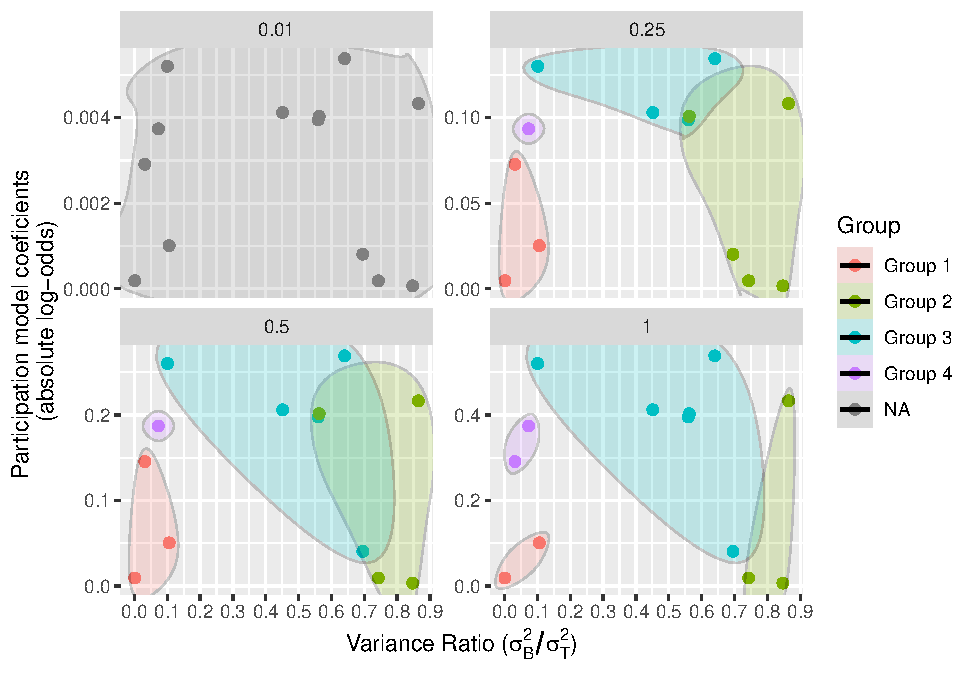
\includegraphics{5---Analysis_files/figure-latex/unnamed-chunk-37-1.pdf}
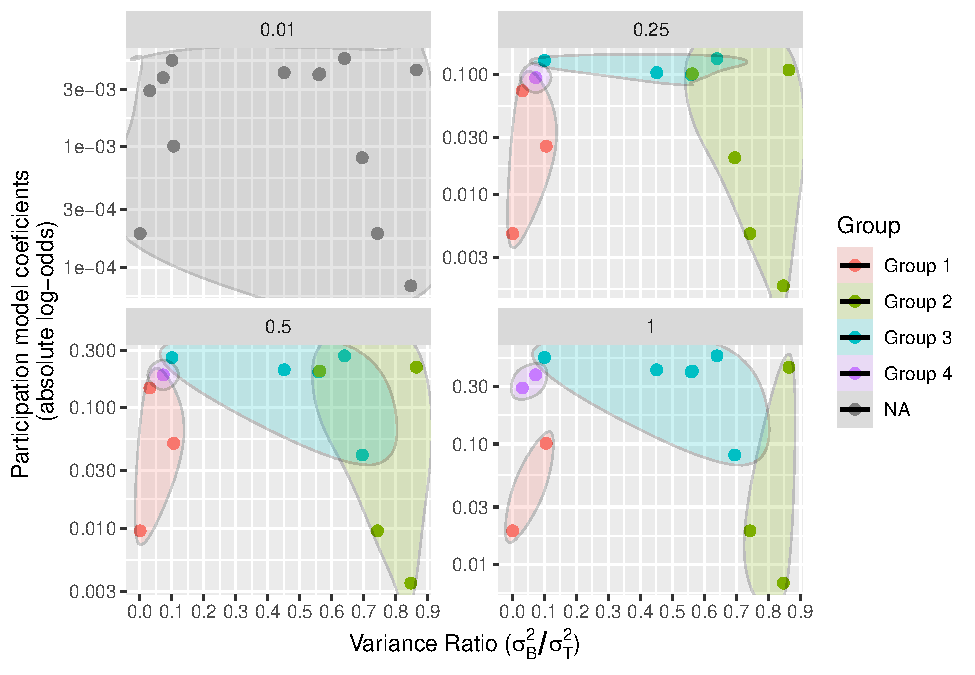
\includegraphics{5---Analysis_files/figure-latex/unnamed-chunk-38-1.pdf}

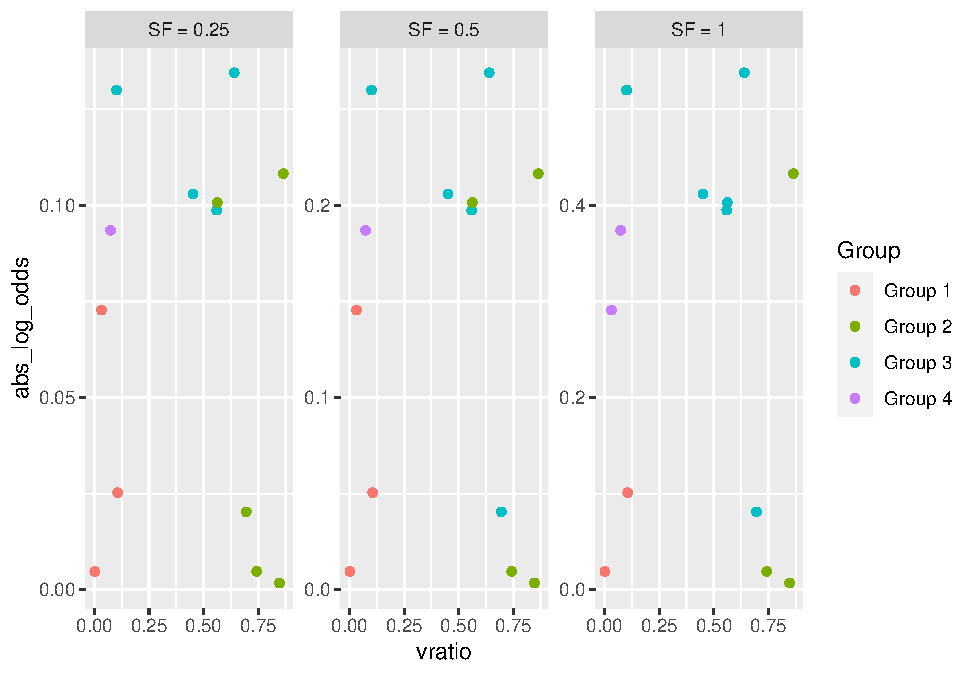
\includegraphics{5---Analysis_files/figure-latex/unnamed-chunk-39-1.pdf}

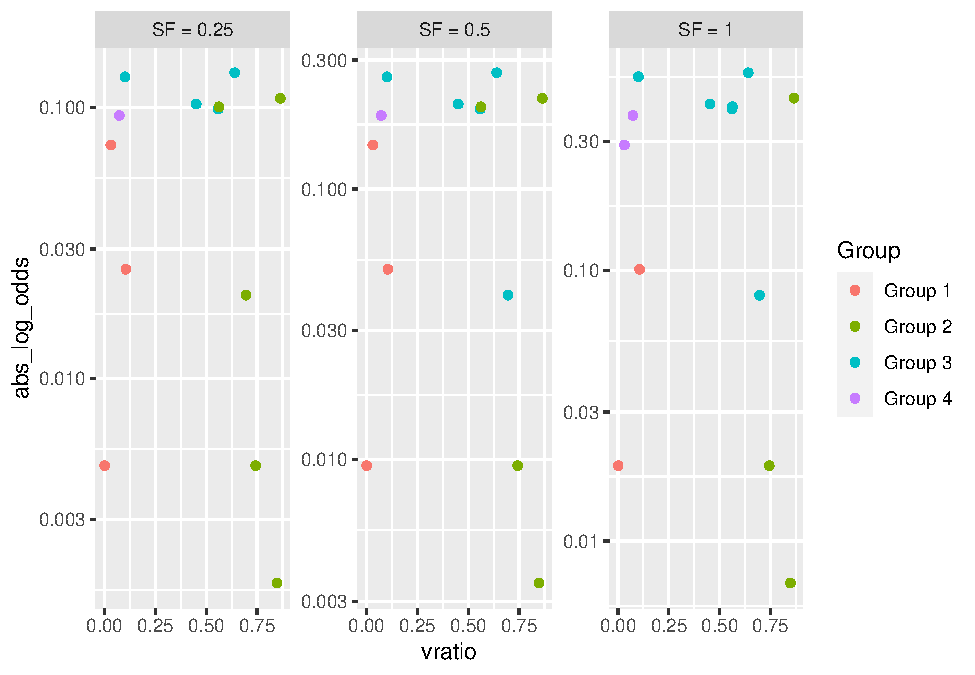
\includegraphics{5---Analysis_files/figure-latex/unnamed-chunk-40-1.pdf}

\hypertarget{test-1---same-abs_log_odds}{%
\paragraph{Test 1 - same abs\_log\_odds}\label{test-1---same-abs_log_odds}}

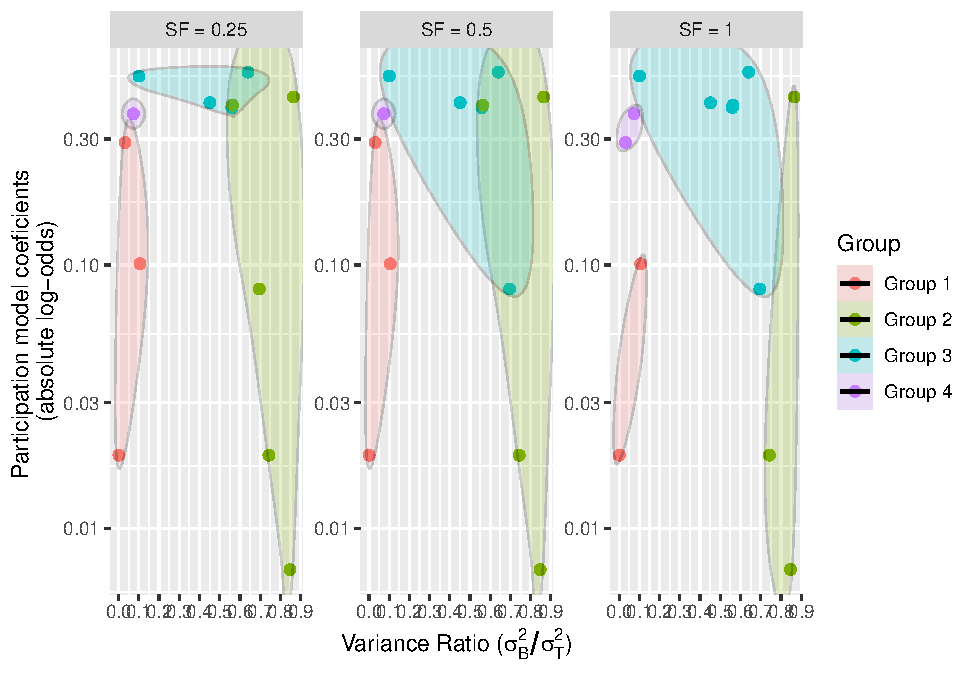
\includegraphics{5---Analysis_files/figure-latex/unnamed-chunk-41-1.pdf}
\#\#\#\# Test 2 - relative log\_odds and relative vratio

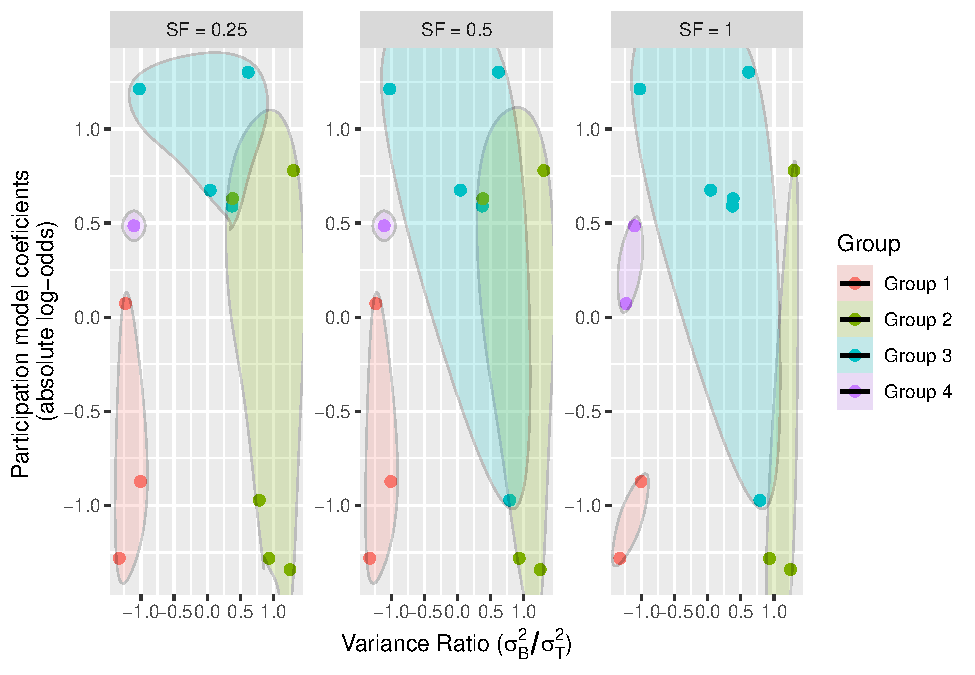
\includegraphics{5---Analysis_files/figure-latex/unnamed-chunk-43-1.pdf}

\hypertarget{feasibility}{%
\subsection{Feasibility}\label{feasibility}}

\hypertarget{sampling-difficulty}{%
\subsubsection{Sampling Difficulty}\label{sampling-difficulty}}

\hypertarget{sf-1}{%
\paragraph{SF = 1}\label{sf-1}}

\begin{figure}
\centering
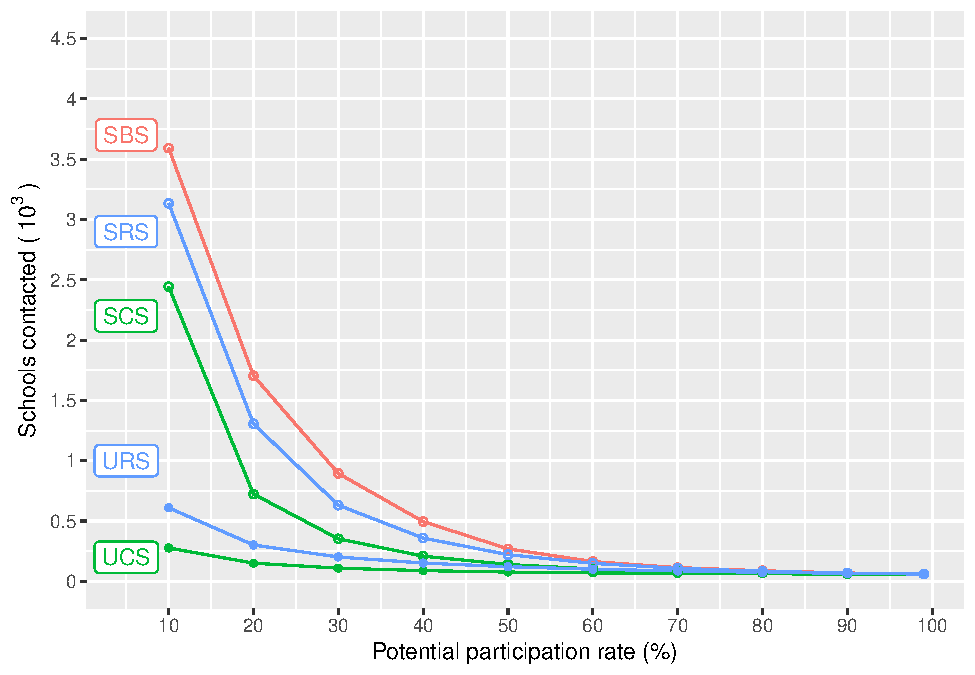
\includegraphics{5---Analysis_files/figure-latex/unnamed-chunk-45-1.pdf}
\caption{\label{fig:unnamed-chunk-45}Schools Contacted}
\end{figure}

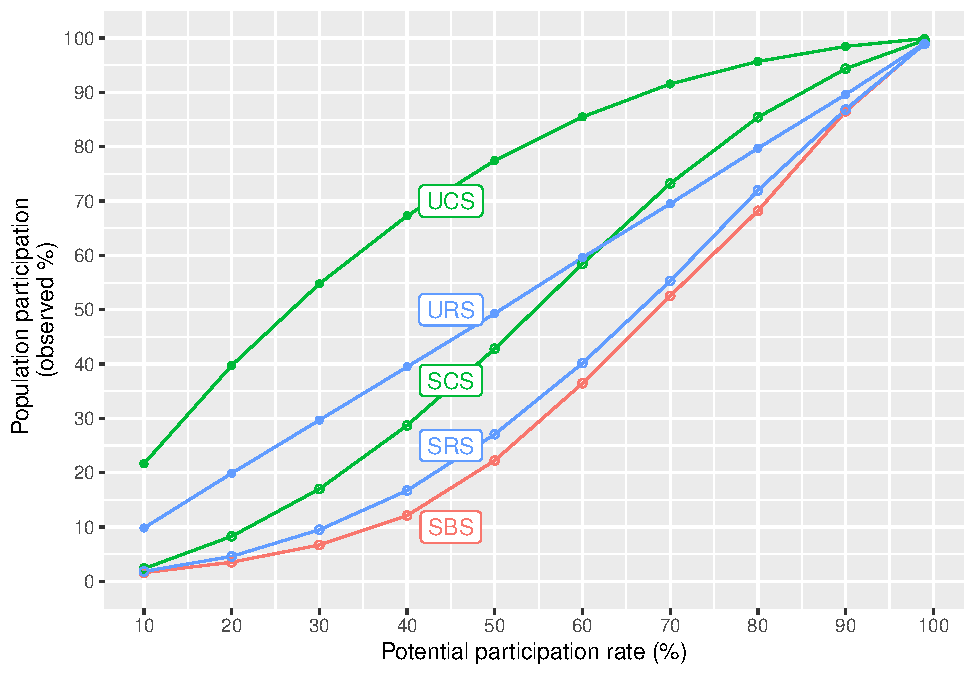
\includegraphics{5---Analysis_files/figure-latex/unnamed-chunk-46-1.pdf}
\#\#\#\# SF = {[}1, .5, .25, .01{]}

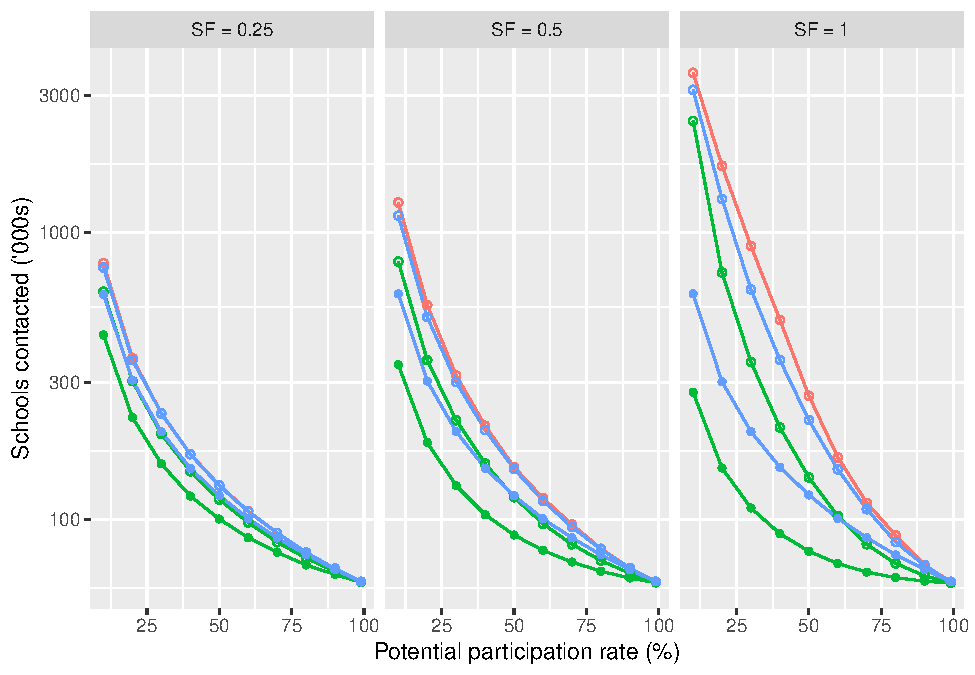
\includegraphics{5---Analysis_files/figure-latex/unnamed-chunk-47-1.pdf}

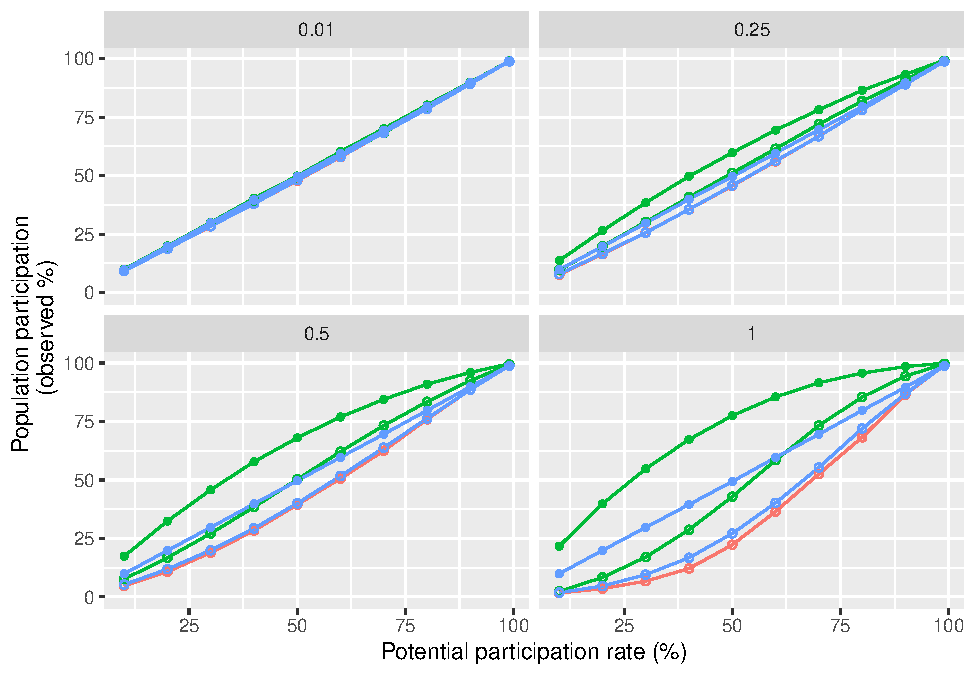
\includegraphics{5---Analysis_files/figure-latex/unnamed-chunk-48-1.pdf}

\hypertarget{difficulty-relative-to-comparison-methods}{%
\subsubsection{Difficulty Relative to Comparison Methods}\label{difficulty-relative-to-comparison-methods}}

\hypertarget{sf-1-1}{%
\paragraph{SF = 1}\label{sf-1-1}}

\includegraphics{5---Analysis_files/figure-latex/unnamed-chunk-50-1.pdf}

\includegraphics{5---Analysis_files/figure-latex/unnamed-chunk-51-1.pdf}

\hypertarget{sf-1-.5-.25-.01}{%
\paragraph{SF = {[}1, .5, .25, .01{]}}\label{sf-1-.5-.25-.01}}

\includegraphics{5---Analysis_files/figure-latex/unnamed-chunk-52-1.pdf}
\#\#\# Gini Plot

\includegraphics{5---Analysis_files/figure-latex/unnamed-chunk-54-1.pdf}

\hypertarget{export-data}{%
\section{Export Data}\label{export-data}}

\hypertarget{a-tibble-28-x-2}{%
\section{A tibble: 28 x 2}\label{a-tibble-28-x-2}}

Vars MB\\
\strut \\
1 tabs 473.62 Mb
2 figs 301.614 Mb
3 results 84.955 Mb
4 df.list 19.796 Mb
5 df.sim 3.027 Mb\\
6 plot\_smd 0.077 Mb\\
7 test.group 0.066 Mb\\
8 df.smd.ipsw 0.038 Mb\\
9 get\_quant 0.03 Mb\\
10 test 0.013 Mb\\
\# \ldots{} with 18 more rows
\# A tibble: 20 x 2
fig size\\
\strut \\
1 dist 263.1 Mb
2 ch 0 Mb\\
3 vratio 0 Mb\\
4 allocation 0 Mb\\
5 joint.cluster.stats 0 Mb\\
6 cluster.SMD 0.2 Mb\\
7 B 0.1 Mb\\
8 smd.by.scale 0.4 Mb\\
9 smd.examples 0.1 Mb\\
10 smd.examples.sf100 0 Mb\\
11 v.coef 0 Mb\\
12 samples.contacts.sf100 0 Mb\\
13 samples.response.rates.sf100 0 Mb\\
14 samples.contacts.sf.all 0 Mb\\
15 samples.response.rates.sf.all 0 Mb\\
16 relative.counts.URS 0 Mb\\
17 relative.counts.UCS 0 Mb\\
18 samples.relative.contacts.sf.all 0 Mb\\
19 gini 0 Mb\\
20 gini.coef 37.4 Mb
\# A tibble: 16 x 2
tab size\\
\strut \\
1 pop.desc 0 Mb\\
2 dist 263.1 Mb
3 allocation 0 Mb\\
4 cluster.SMD 0.2 Mb\\
5 strata.data 0 Mb\\
6 intercepts 0 Mb\\
7 B 0 Mb\\
8 smd.results 0.2 Mb\\
9 smd.by.scale 0.6 Mb\\
10 smd.examples 0.1 Mb\\
11 samples 0 Mb\\
12 samples.contacts.labels.sf100 0 Mb\\
13 samples.response.rates.labels.sf100 0 Mb\\
14 relative.counts 0.1 Mb\\
15 gini.coef 0 Mb\\
16 gini.count 209.2 Mb

\hypertarget{presentation-figures}{%
\section{Presentation Figures}\label{presentation-figures}}


\end{document}
